\documentclass[11pt,a4paper]{article}
\usepackage[utf8]{inputenc}
\usepackage{color}
\usepackage{enumerate}
\usepackage{fancyhdr}
%\usepackage{minted}
\usepackage{graphicx}
\usepackage{array}
\usepackage{hyperref}
\usepackage{amssymb}
\usepackage{multirow}
\usepackage{morefloats}
\usepackage{amsmath}
\usepackage{titlesec}
\usepackage[spanish]{babel}
\usepackage[spanish]{algorithm2e}
\usepackage[table]{xcolor}
\usepackage{anysize}
\usepackage[section]{placeins}
\usepackage{graphicx}
\usepackage{mathtools}
\usepackage{amsmath}


\hypersetup{
	colorlinks,
	citecolor=black,
	filecolor=black,
	linkcolor=black,
	urlcolor=blue
}

\newcommand{\horrule}[1]{\rule{\linewidth}{#1}}

\title{
	\normalfont \normalsize 
	\textsc{\textbf{Metaheurísticas (2016-2017)} \\ Grado en Ingeniería Informática \\ Universidad de Granada} \\ [25pt] % Your university, school and/or department name(s)
	\horrule{0.5pt} \\[0.4cm] % Thin top horizontal rule
	\huge Trabajo Final: Búsqueda por Vórtices  \\ % The assignment title
	\horrule{2pt} \\[0.5cm] % Thick bottom horizontal rule
}

\author{Germán González Almagro} % Nombre y apellidos

\marginsize{3cm}	% margen izquierdo
{3cm}				% margen derecho
{1.2cm}				% margen superior
{1.5cm} 			% margen inferior

%\titleformat{\section}{\normalfont\LARGE}{}{0pt}{\bfseries\LARGE}

\begin{document}
	
	\date{\today}
	
	\maketitle
	
	\vspace{1cm}
	
	\begin{figure}[!h]
		\centering
		
\includegraphics[scale=0.4]{LogoUGR.png} 
	\end{figure}
		
	\newpage
	
	\tableofcontents
	
%	\listoffigures
	
%	\listoftables
	
	\newpage
	
\section{Descripción de la Búsqueda por Vórtices}

	\noindent La búsqueda por vórtices (Vortex Search) es un método de optimización algorítmica desarrollado por Berat Dogan y Tamer Olmez, profesores de la Universidad Técnica de Estambul. Como ya viene siendo frecuente en este tipo de métodos, se trata de un algoritmo bioinspirado, que emplea los vórtices de agua como método para guiar el proceso de búsqueda del óptimo.\\
	
	\noindent La búsqueda por vórtices es un método basado en trayectorias simples, que se vale de un mecanismo que imita los vórtices de agua para evitar la localidad en el proceso de búsqueda. Este proceso consiste en generar una nube de puntos, según una distribución Gaussiana o normal, contenida en una circunferencia, cuyo radio disminuye con el paso de las iteraciones. De esta forma, en cada iteración se evalúan los puntos generados y se selecciona el mejor encontrado hasta el momento como centro de la nueva circunferencia, siempre de radio menor que la anterior. La siguiente imagen muestra esta idea:
	
	\begin{figure}[!h]
		\centering
		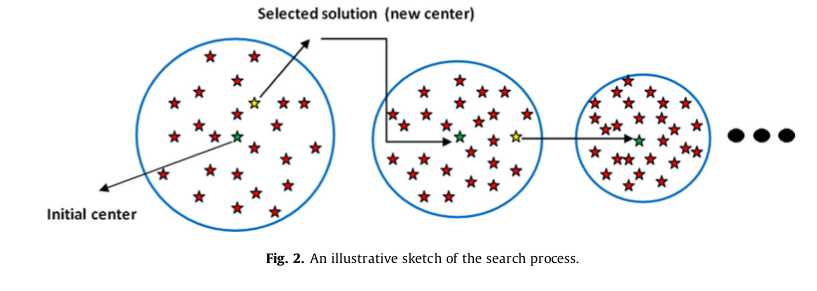
\includegraphics[scale=0.45]{Imagenes/Imagen1.png} 
		\caption{Descripción gráfica del proceso de búsqueda.} \label{fig:figura2}
	\end{figure} 
	
	\noindent En el proceso de búsqueda descrito podemos diferenciar dos partes, la parte de exploración y la de explotación, la primera corresponde a las fases en las que el radio de la hiperesfera que describe el estado del vórtice es lo suficientemente grande en el espacio como para abarcar mas de un óptimo, y por tanto el proceso de búsqueda es susceptible de considerarlos como nuevo óptimo global, mientras que el segundo corresponde a las fases en las que el radio es menor y por tanto se busca explotar al máximo el óptimo encontrado en la fase de exploración. La siguiente gráfica muestra el proceso de decremento del radio: 
	
	\begin{figure}[!h]
		\centering
		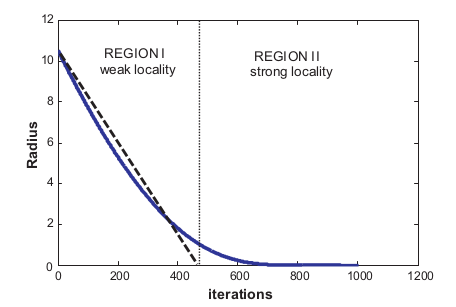
\includegraphics[scale=0.55]{Imagenes/Imagen2.png} 
		\caption{Gráfica que muestra los cambios en el valor del radio.} \label{fig:figura2}
	\end{figure}
	
	\clearpage
	
	\noindent Con esto, obtenemos un algoritmo basado en trayectorias simples capaz de considerar más de un óptimo de la función como mejor objetivo a alcanzar y, por tanto, evitar en cierta medida la localidad. El pseudocódigo del algoritmo es el siguiente:
	
	\begin{algorithm}
		
		\KwIn{Dados $Psize$, el número de nuevas soluciones que se generan en cada iteración,
			$LimSup$, el límite superior de la función objetivo, $LimInf$, el límite superior de la función objetivo, y $MaxIters$, el número máximo de iteraciones.}
		\textbf{function} $VortexSearch(Psize, \; LimSup, \; LimInf,\; MaxIters)$
		\Begin{
			$\mu \leftarrow 0.5 \times (LimSup + LimInf) $\\
			$Centro \leftarrow [\mu \cdots \mu]$ \texttt{\#$|Centro| = Dimension$}\\
			
			$ginv \leftarrow \frac{1}{0.1}*gammaincinv(0.1,\frac{MaxIters-1}{MaxIters})$\\
			
			$Radio = ginv \times \frac{LimSup - LimInf}{2}$\\
			
			$Count \leftarrow max\_iters$\\
			
			\texttt{\#Generamos las soluciones candidatas usando una Gaussiana alrededor del centro}\\
			
			\While{$Count > 0$}{
				
				\texttt{\#Generamos una nube de $Psize$ puntos empleando una Gaussiana}\\
				
				$C \leftarrow Radio \times Gaussian(Psize,\; Dimension)$\\
				
				\texttt{\#Desplazamos la nube de puntos hacia el centro actual}\\
				
				$C_s \leftarrow C + Centro$\\
				
				\texttt{\#Truncamos los valores que se salgan de los límites}\\
				
				$C_s \leftarrow Limitar(C_s, LimSup, LimInf)$\\
				
				\texttt{\#Evaluamos las soluciones candidatas}\\
				
				$Evals \leftarrow FuncionObjetivo(C_s)$\\
				
				\texttt{\#Buscamos el mejor valor de entre los obtenidos}\\
				
				$MejorValor \leftarrow Min(Evals)$\\
				
				\texttt{\#Actualizamos la mejor solución si fuese necesario}\\
				
				\If{$MejorValor < OptGlobal$}{
					$OptGlobalValor \leftarrow MejorValor$\\
					$OptGlobalSolucion \leftarrow Index(MejorValor)$\\
					
				}
				
				\texttt{\#El centro es siempre establecido al mejor valor hasta el momento}\\
				
				$Centro \leftarrow OptGlobalSolucion$\\
				
				\texttt{\#Actualizamos el contador y el radio}\\
				
				$Count \leftarrow Count - 1; \;\; a \leftarrow \frac{Count}{MaxIters}$\\
				$ginv \leftarrow \frac{1}{0.1}*gammaincinv(0.1,a)$\\
				$Radio = ginv \times \frac{LimSup - LimInf}{2}$\\
				
			}
			
			\KwRet $OptGlobalSolucion$\\
		}
		
	\end{algorithm}	
	
	\noindent Donde la función $gammaincinv()$ es la función Gamma Incompleta Inversa, empleada para calcular la actualización del radio en cada iteración, y definida como la inversa de la siguiente expresión:
	
	$$ \gamma(x,a) = \int_{0}^{x} e^{-t}t^{a-1}dt \;\; t.q. \; a > 0$$
	
\section{Experimentación}

	\noindent Para evaluar la calidad del algoritmo optimizaremos 12 funciones empleadas en la competición de 2005 (ver anexo 1), para dimensiones 20 y 30. Calcularemos para cada caso la desviación respecto del óptimo, de esta forma obtendremos un resultado que no depende del valor del óptimo en sí, sino del ajuste proporcionado por el algoritmo. La siguiente tabla muestra, para cada caso, el valor del óptimo, el valor obtenido mediante la búsqueda por vórtices y la desviación del valor obtenido respecto del óptimo trabajando en dimensión 10:\\
	
	\begin{table}[h]
		\centering
		\setlength{\arrayrulewidth}{1mm}
		\setlength{\tabcolsep}{10pt}
		\renewcommand{\arraystretch}{1.1}
		
		\rowcolors{2}{gray!25}{white}
		\begin{tabular}{ >{\centering\arraybackslash}m{1.15cm}  >{\centering\arraybackslash}m{1.2cm}  >{\centering\arraybackslash}m{1.2cm}   >{\centering\arraybackslash}m{1.4cm}  >{\centering\arraybackslash}m{1.15cm}  >{\centering\arraybackslash}m{1.2cm}  >{\centering\arraybackslash}m{1.2cm}   >{\centering\arraybackslash}m{1.4cm}  }
			\hline
			\rowcolor{black}
			\multicolumn{8}{c}{\bf \color{white}{Vortex Search (Dimension 10)}}\\
			\hline
			\rowcolor{gray!50}
			\textbf{Función} & \textbf{Valor} & \textbf{Optimo} & \textbf{Desv.} & \textbf{Función} & \textbf{Valor} & \textbf{Optimo} & \textbf{Desv.} \\
			F1 & -450.0 & -450.0 & 0.0 & F10  & -308.11 & -330.0 & 6.633  \\
			F2 & -450.0 & -450.0 & 0.0 & F11  & 91.72 & 90.0 & 1.9162   \\
			F5 & -285.62 & -310.0 & 7.8655 & F13  & -127.47 & -130.0 & 1.942 \\
			F6 & 395.507 & 390.0 & 1.4121 & F14 & -296.86 & -300.0 & 1.046 \\
			F8 & -119.99 & -140.0 & 14.288 & F17 & 166.44 & 120.0 & 38.7 \\
			F9 & -314.08 & -330.0 & 4.824 & F24  & 460.0 & 260.0 & 76.9231 \\
			
			\hline
			
		\end{tabular}
		
	\end{table}
	
	\noindent A la vista de los resultados podemos decir que, como era de esperar, la búsqueda por vórtices obtiene el óptimo para el problema en los casos en los que este está bien diferenciado, ya sea porque no hay óptimos locales, o porque estos están lo suficientemente alejados del óptimo local como para interferir en el proceso de búsqueda. Por otra parte, en las funciones mas complejas los resultados obtenidos son mejorables, debemos recordar que la búsqueda por vórtices es un algoritmo basado en trayectorias simples y por tanto tiene dificultades al encontrar óptimos globales cuando estos están rodeados por óptimos locales.\\
	
	\noindent La siguiente tabla muestra, para cada caso, el valor del óptimo, el valor obtenido mediante la búsqueda por vórtices, y la desviación del valor obtenido respecto del óptimo trabajando en dimensión 30:\\
	
	\begin{table}[h]
		\centering
		\setlength{\arrayrulewidth}{1mm}
		\setlength{\tabcolsep}{10pt}
		\renewcommand{\arraystretch}{1.1}
		
		\rowcolors{2}{gray!25}{white}
		\begin{tabular}{ >{\centering\arraybackslash}m{1.15cm}  >{\centering\arraybackslash}m{1.2cm}  >{\centering\arraybackslash}m{1.2cm}   >{\centering\arraybackslash}m{1.4cm}  >{\centering\arraybackslash}m{1.15cm}  >{\centering\arraybackslash}m{1.2cm}  >{\centering\arraybackslash}m{1.2cm}   >{\centering\arraybackslash}m{1.4cm}  }
			\hline
			\rowcolor{black}
			\multicolumn{8}{c}{\bf \color{white}{Vortex Search (Dimension 30)}}\\
			\hline
			\rowcolor{gray!50}
			\textbf{Función} & \textbf{Valor} & \textbf{Optimo} & \textbf{Desv.} & \textbf{Función} & \textbf{Valor} & \textbf{Optimo} & \textbf{Desv.} \\
			F1 & -449.98 & -450.0 & 0.0042 & F10 & -121.97 & -330.0 & 63.04  \\
			F2 & -439.55 & -450.0 & 2.32 & F11 & 118.98 & 90.0 & 32.2   \\
			F5 & 11348.48 & -310.0 & 3760.80 & F13 & -109.67 & -130.0 & 15.63 \\
			F6 & 25200.59 & 390.0 & 6361.69 & F14 & -287.03 & -300.0 & 4.32 \\
			F8 & -119.51 & -140.0 & 14.63 & F17 & 113.646 & 120.0 & 5.29 \\
			F9 & -198.58 & -330.0 & 39.822 & F24 & 460.03 & 260.0 & 76.93 \\
			
			\hline
			
		\end{tabular}
		
	\end{table}
	
	\noindent Vemos que, cuando aumentamos el número de dimensiones, el algoritmo sigue dando buenos resultados para las funciones con un óptimo global bien diferenciado. Sin embargo, en algunos casos este aumento en la complejidad de la función a optimizar hace que el algoritmo no sea suficientemente potente como para optimizar funciones que antes si podía.\\
	
	\clearpage
	
	\noindent Para obtener una mejor visión general del comportamiento del algoritmo podemos representar gráficamente el mejor valor obtenido frente al número de evaluaciones realizadas, de esta forma obtenemos las siguientes gráficas:
	
	\begin{figure}[!h]
		\centering
		\begin{minipage}[b]{0.4\textwidth}
			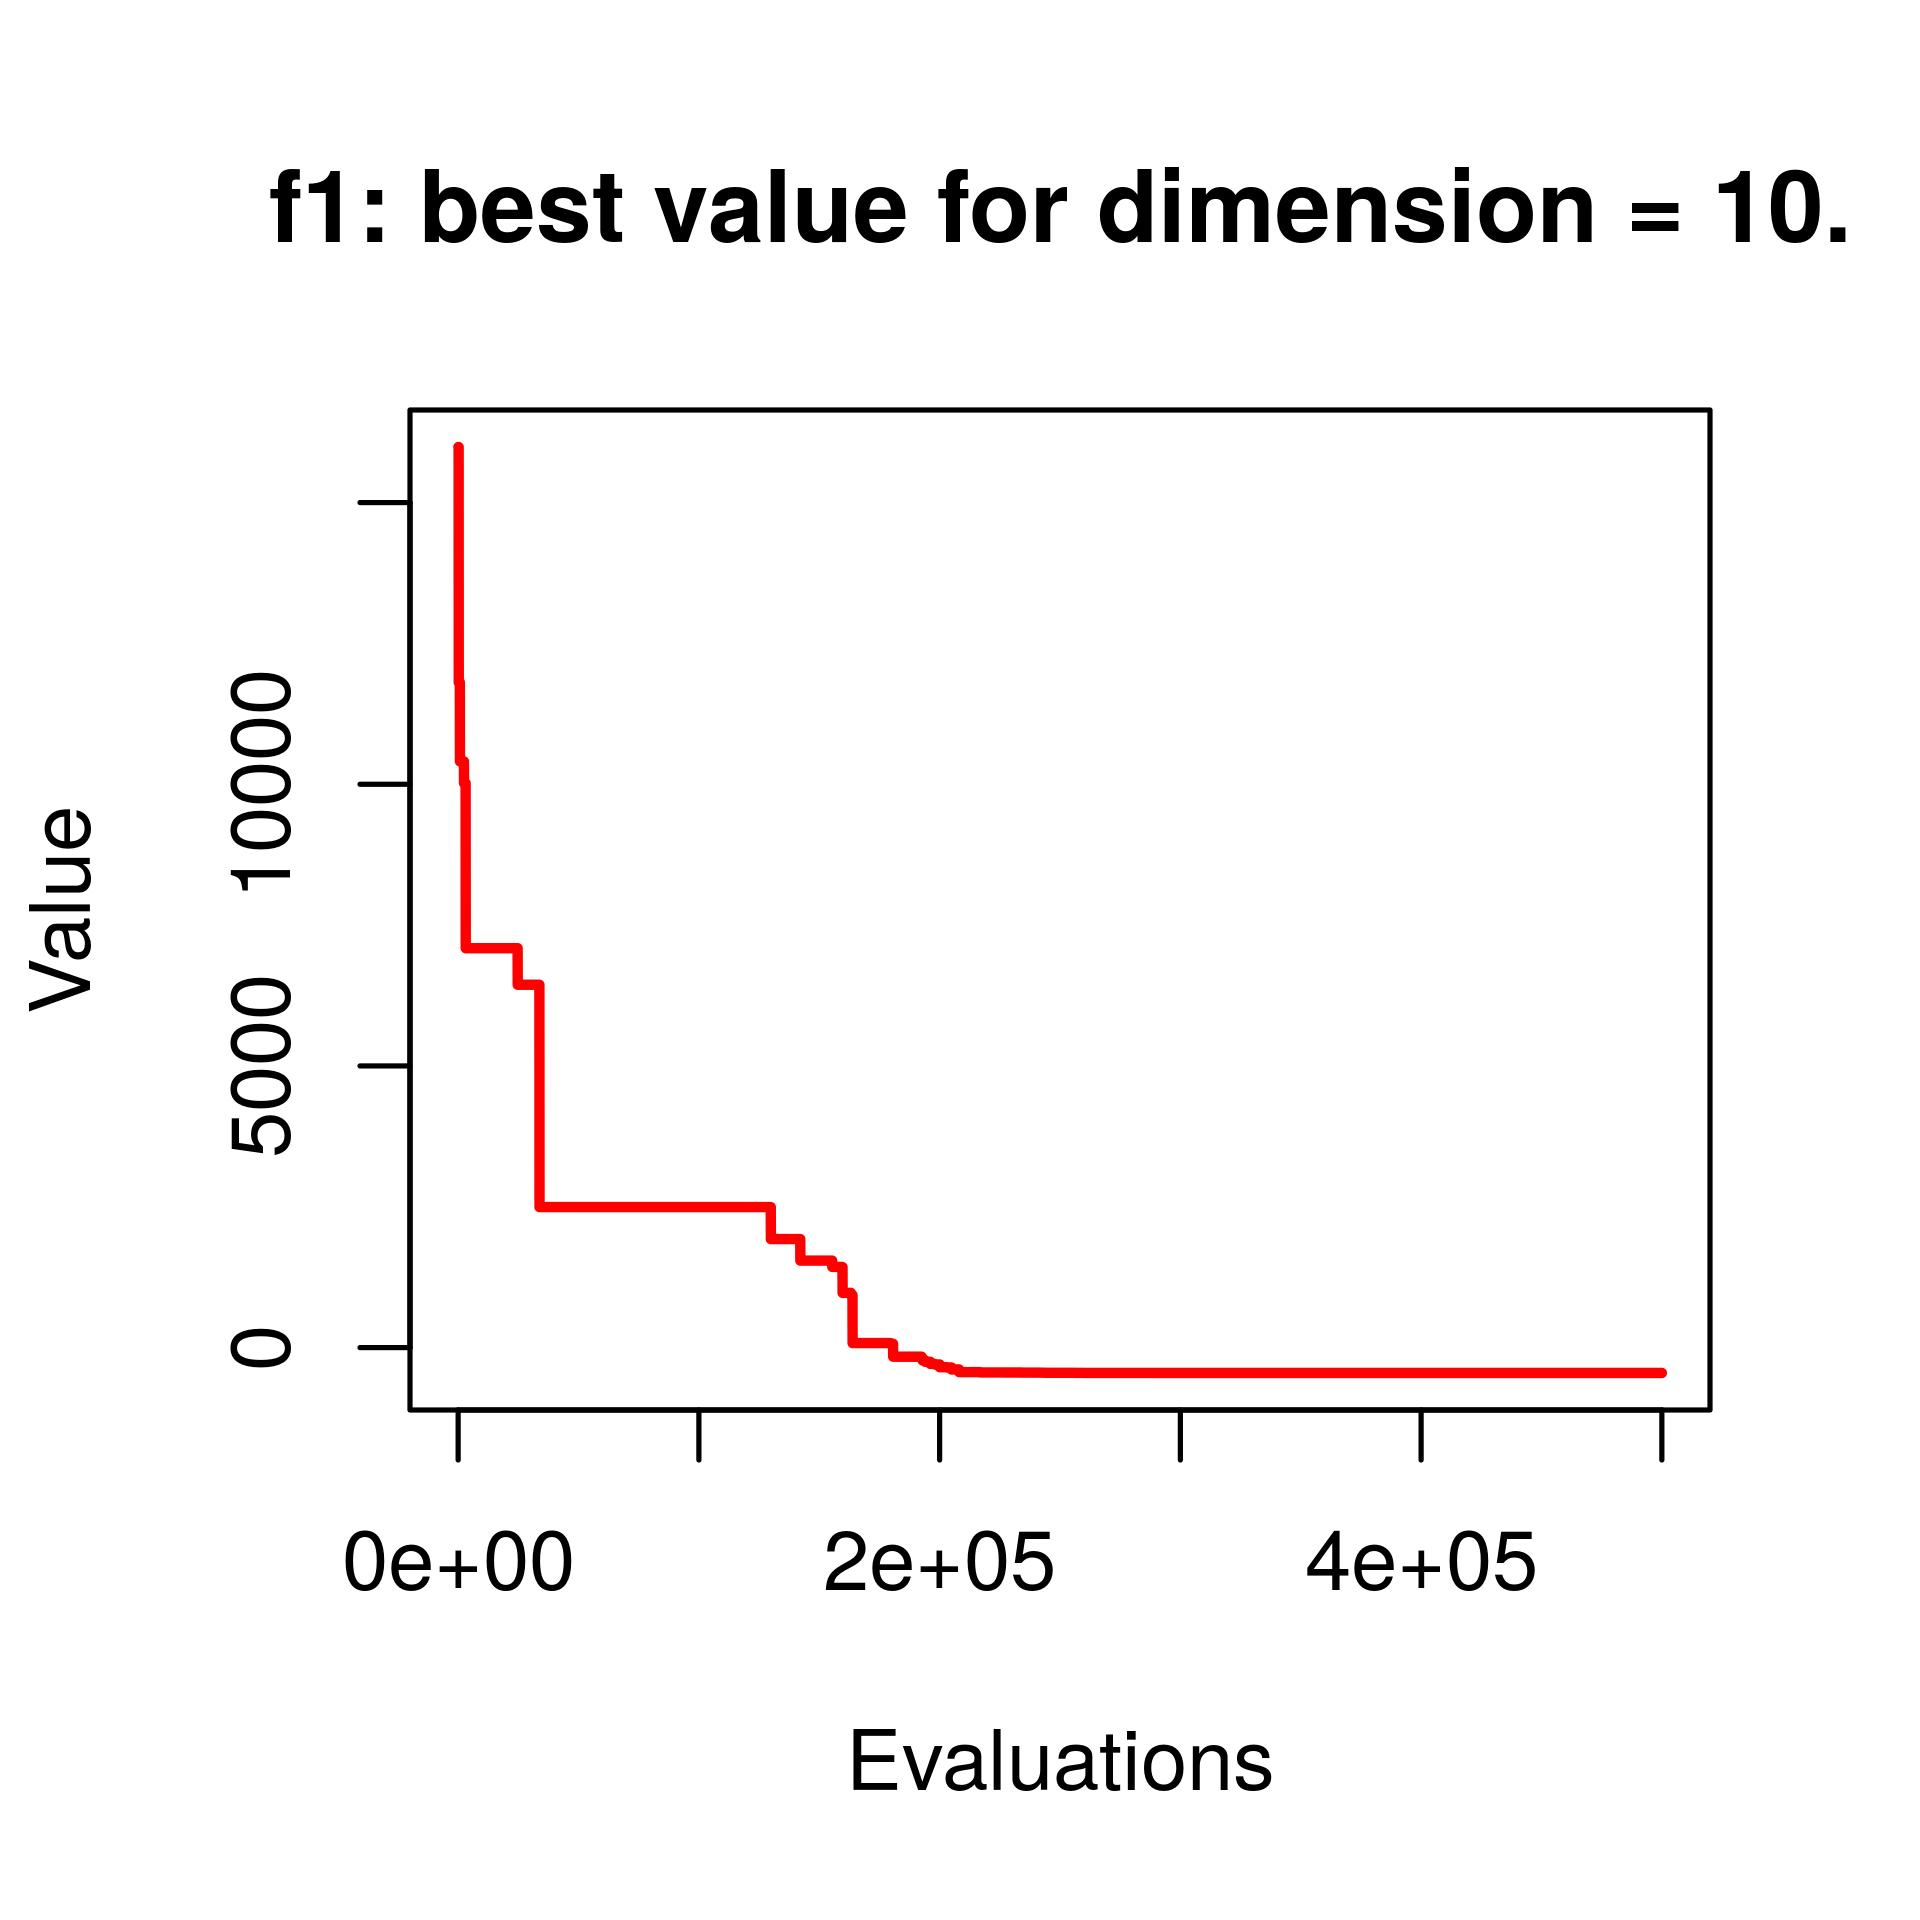
\includegraphics[width=\textwidth]{Imagenes/VS_f1_d10.jpg}
			\caption{Gráfica que representa el mejor valor frente a las evaluaciones para F1 en 10 dimensiones.}
		\end{minipage}
		\hfill
		\begin{minipage}[b]{0.4\textwidth}
			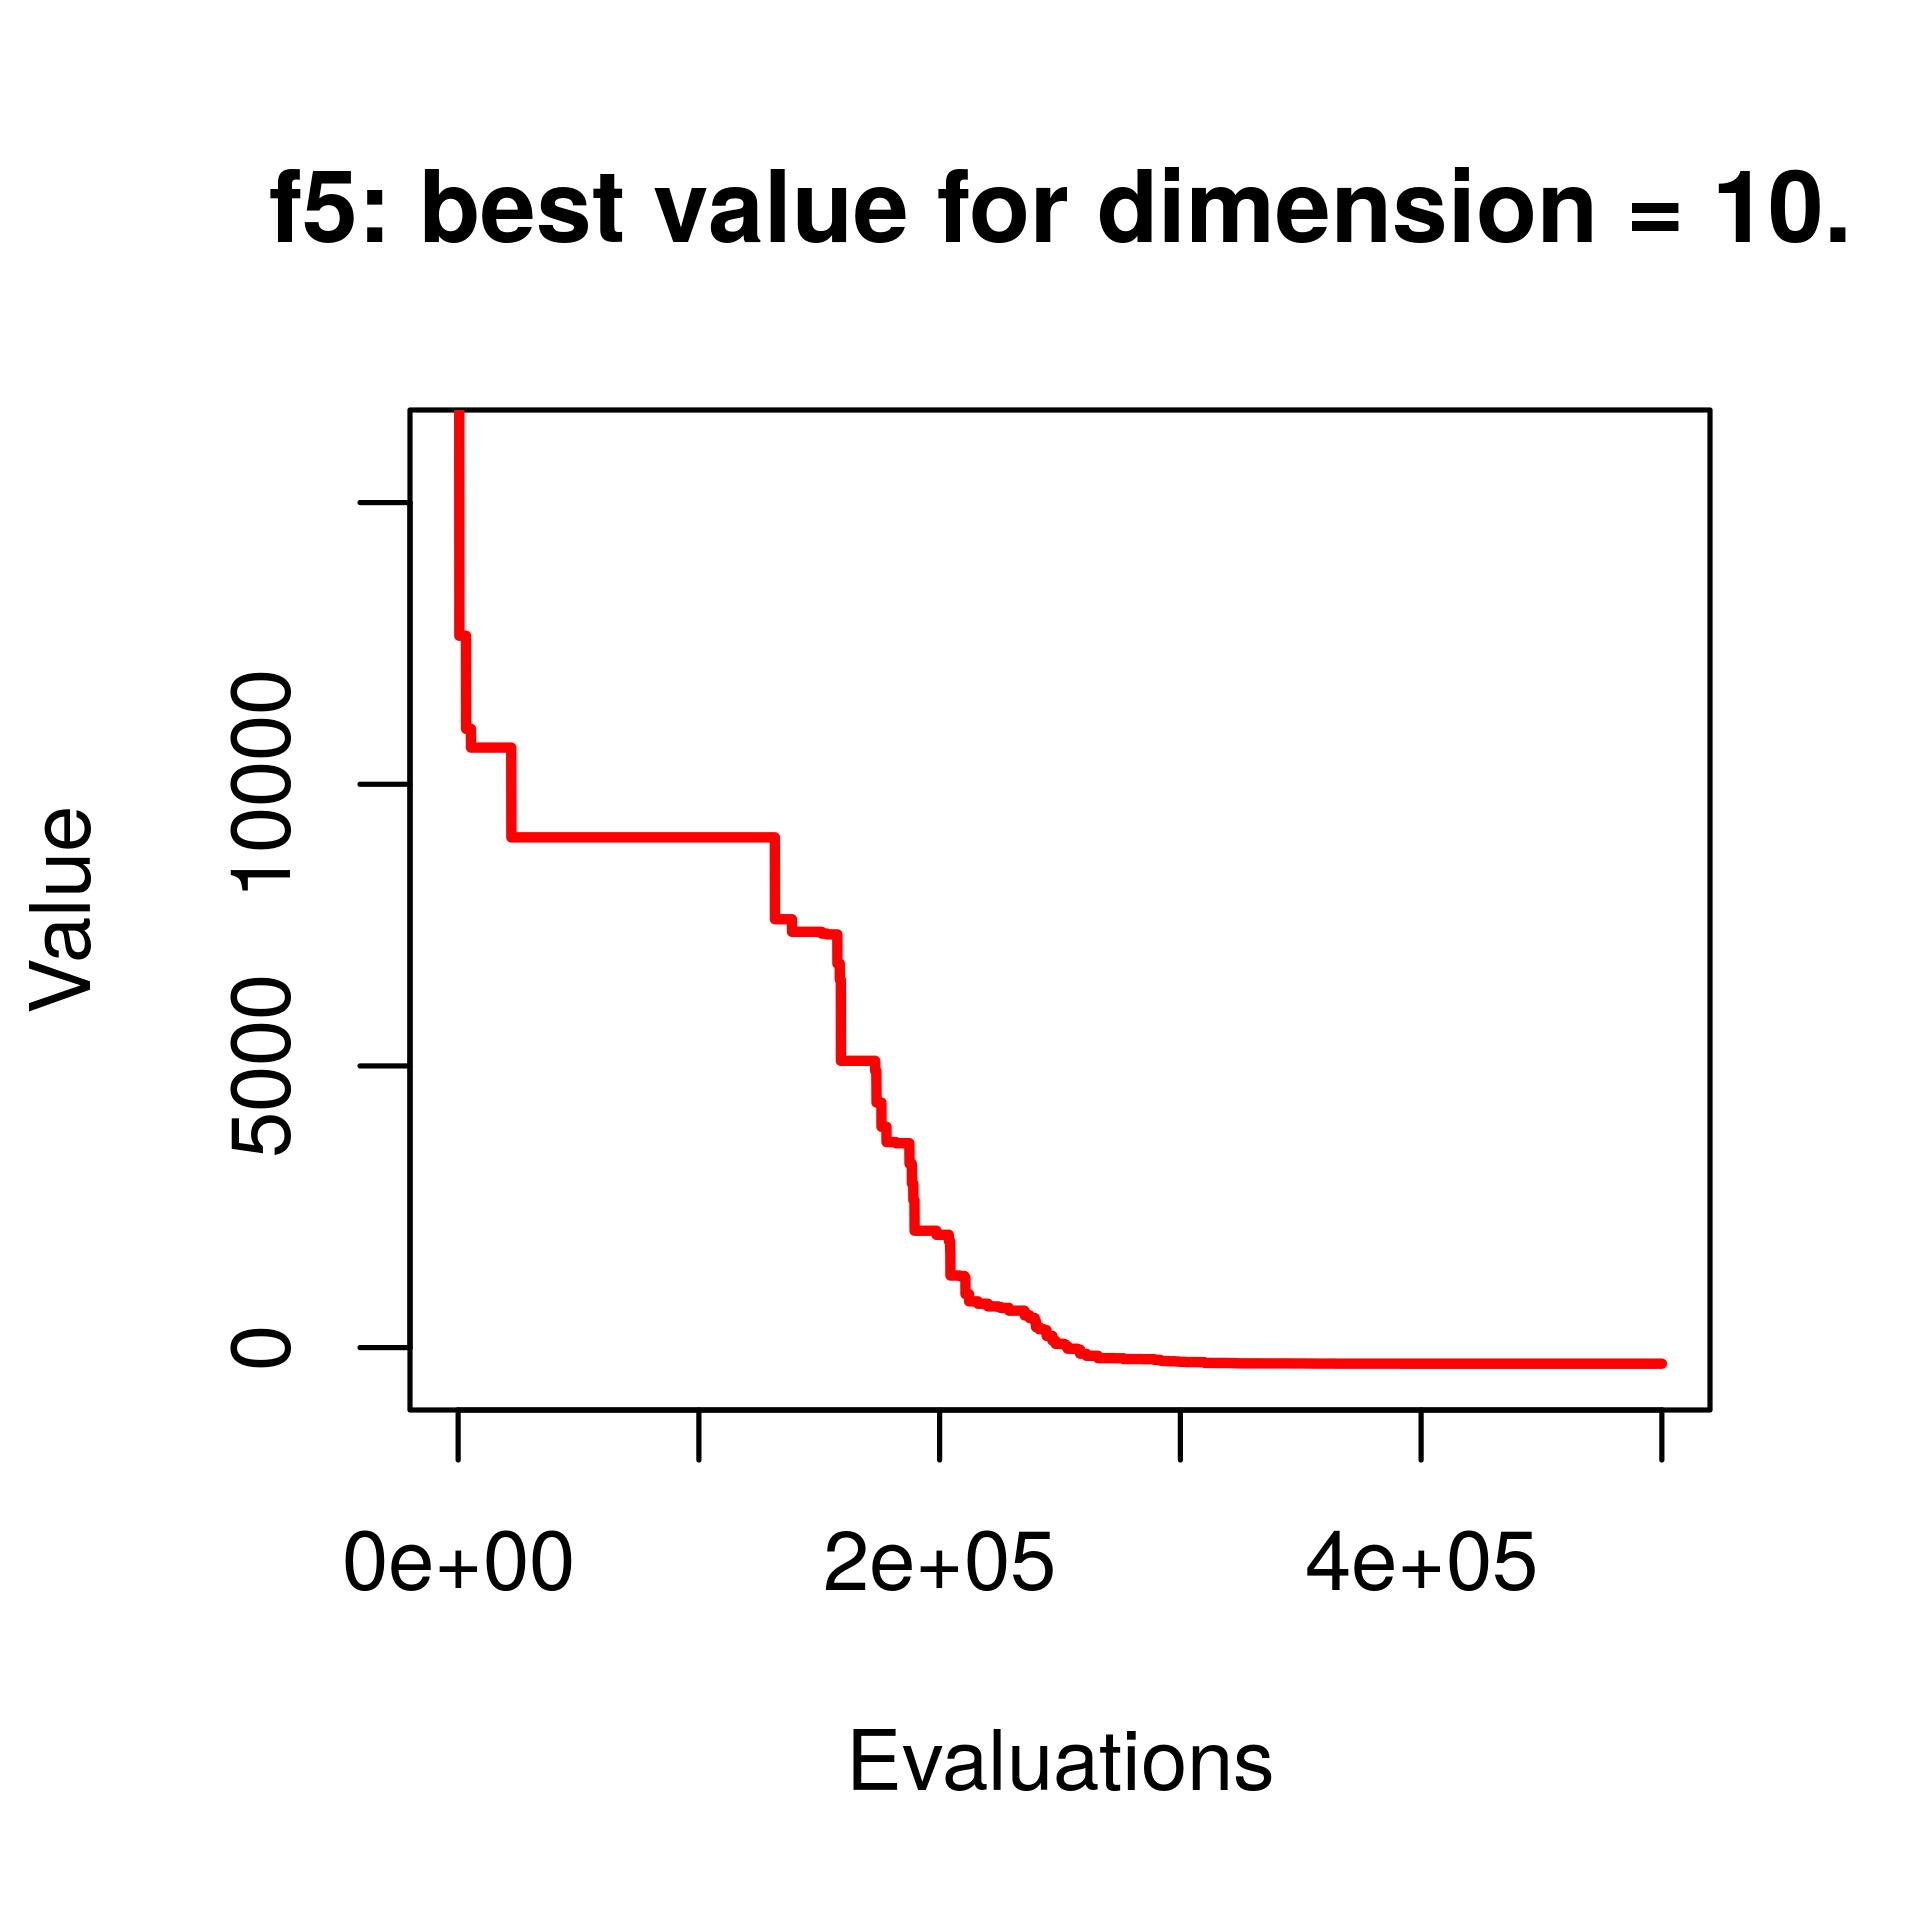
\includegraphics[width=\textwidth]{Imagenes/VS_f5_d10.jpg}
			\caption{Gráfica que representa el mejor valor frente a las evaluaciones para F5 en 10 dimensiones.}
		\end{minipage}
	\end{figure}
	
	\noindent Vemos que, como era de esperar, el mejor valor encontrado por el algoritmo en cada momento disminuye con el paso de las iteraciones, aunque durante algunos periodos se mantiene estable; esto se debe a que en las fases de exploración el algoritmo puede no aceptar una nueva solución como solución actual si ninguna de ellas la mejora, por ello el valor es siempre decreciente y nunca ascendente. Observamos un comportamiento similar al aumentar las dimensiones:
	
	\begin{figure}[!h]
		\centering
		\begin{minipage}[b]{0.4\textwidth}
			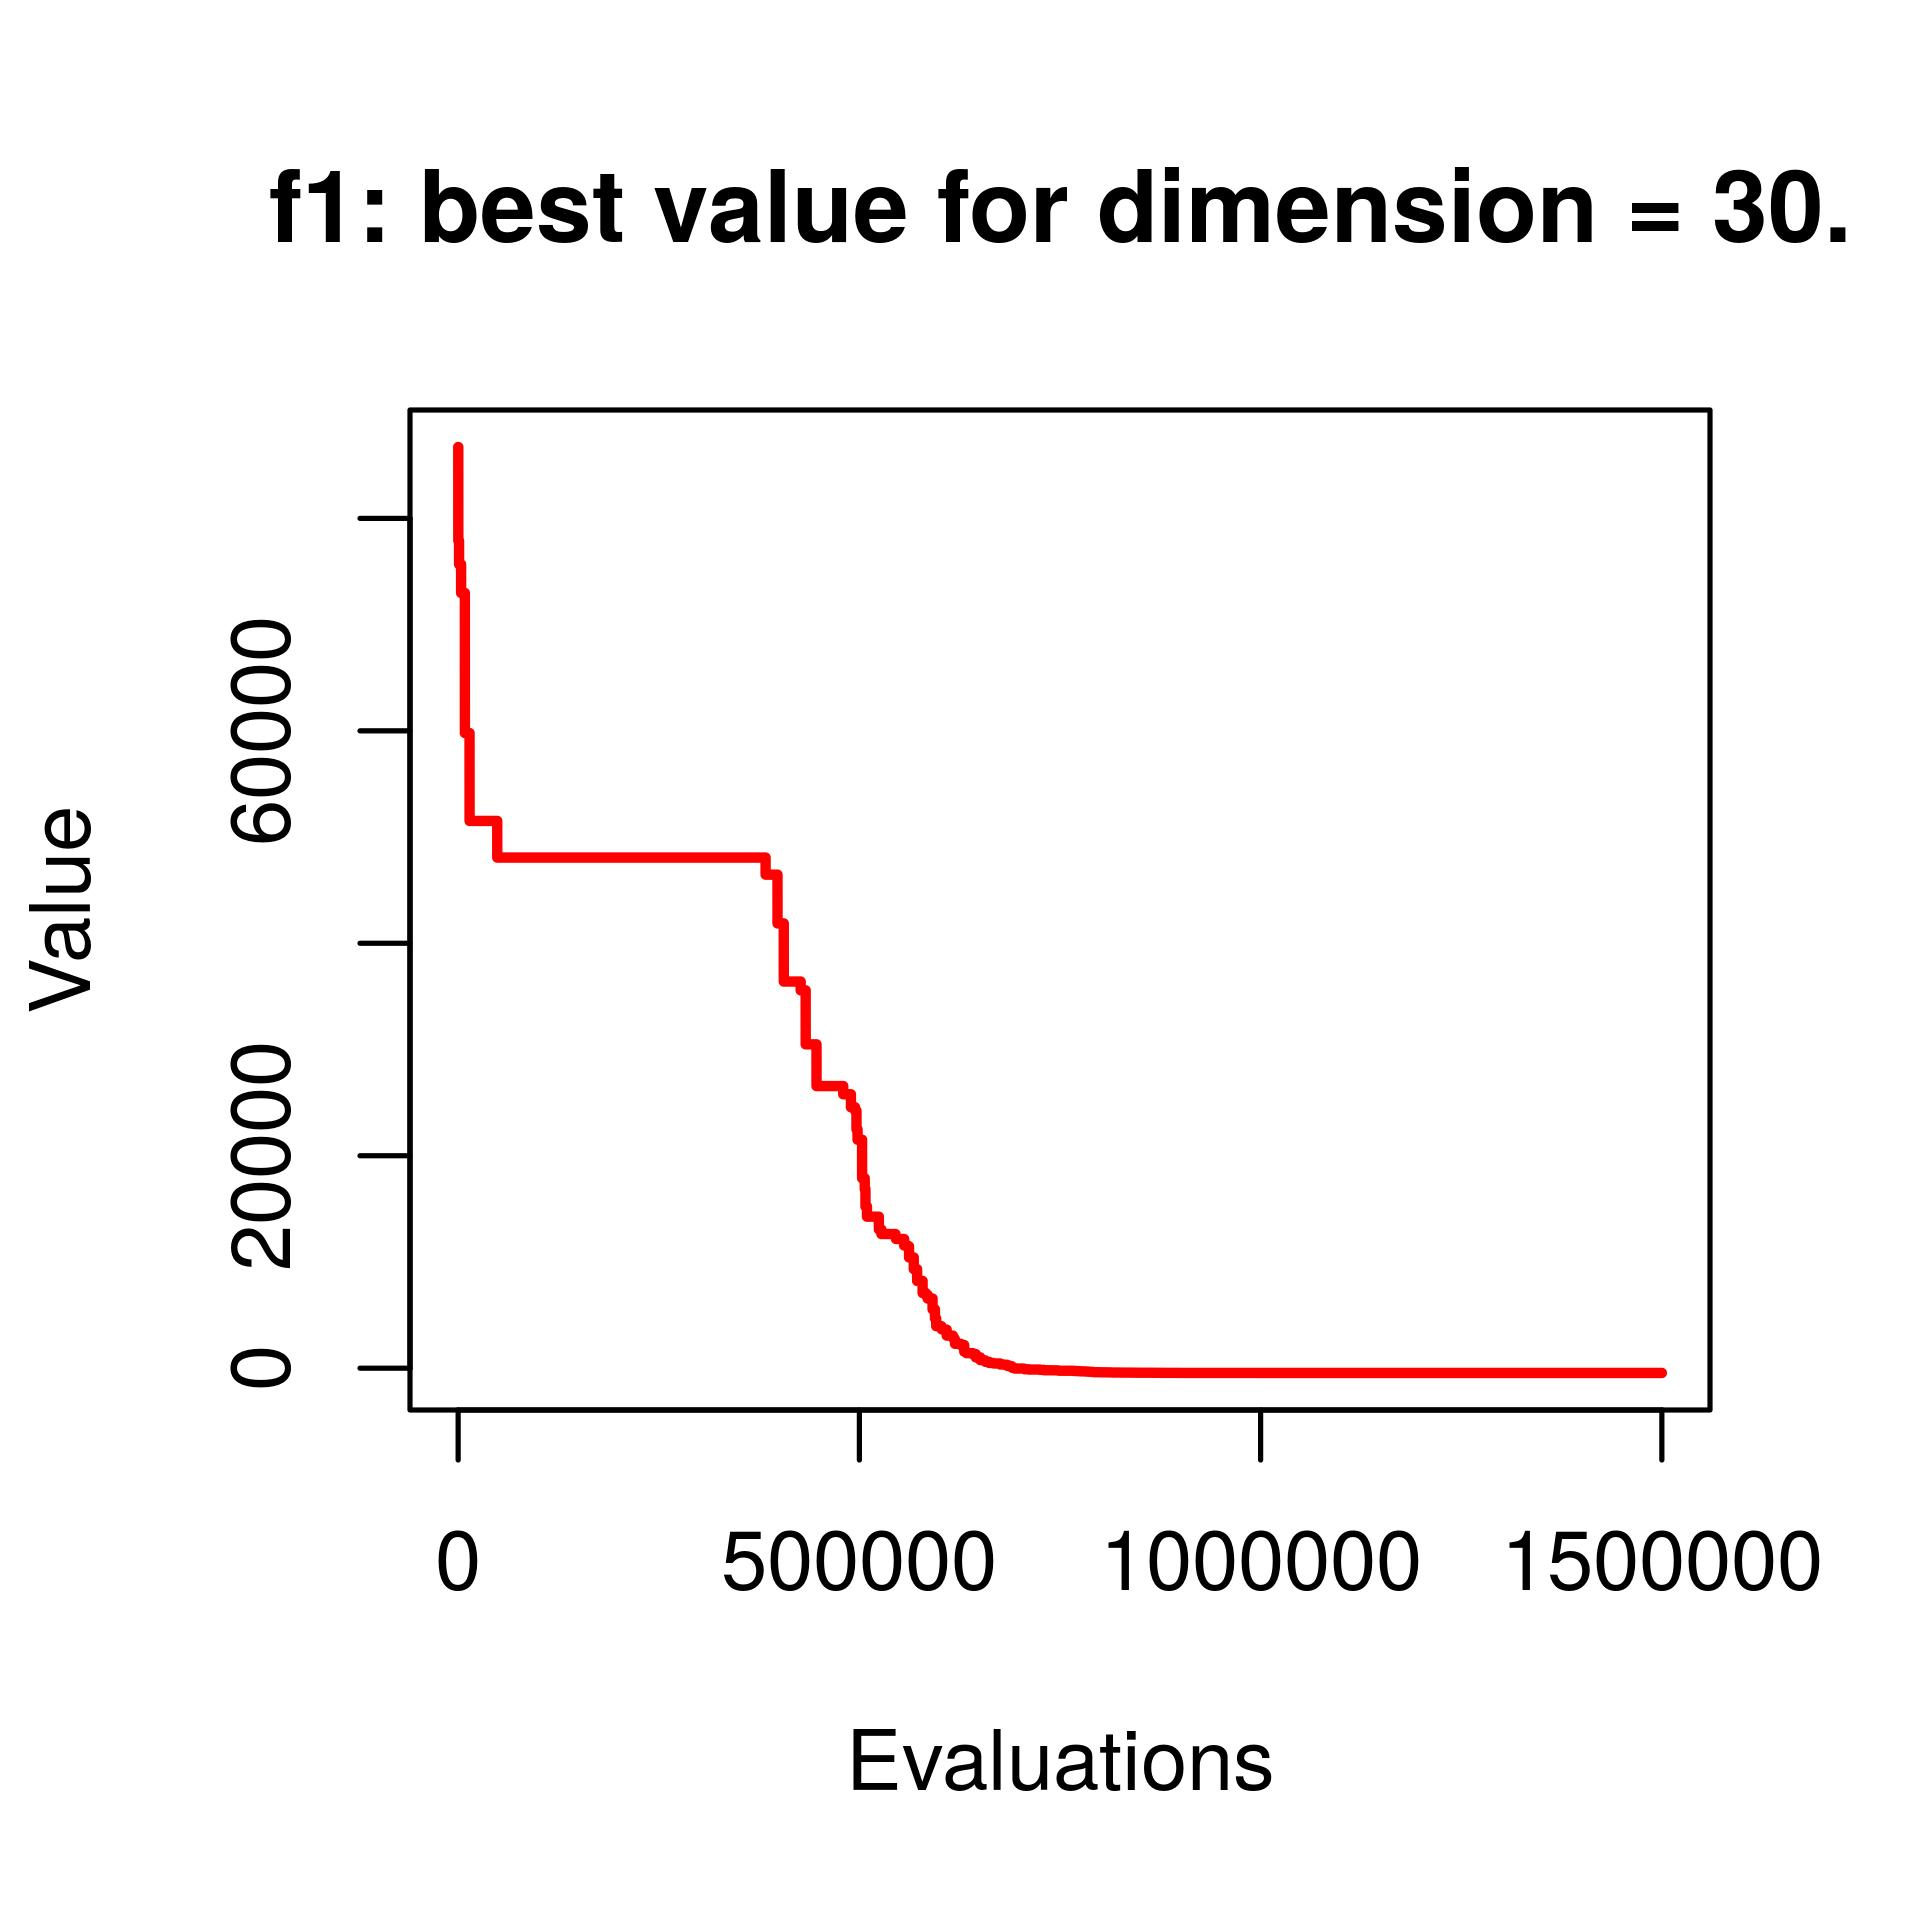
\includegraphics[width=\textwidth]{Imagenes/VS_f1_d30.jpg}
			\caption{Gráfica que representa el mejor valor frente a las evaluaciones para F1 en 30 dimensiones.}
		\end{minipage}
		\hfill
		\begin{minipage}[b]{0.4\textwidth}
			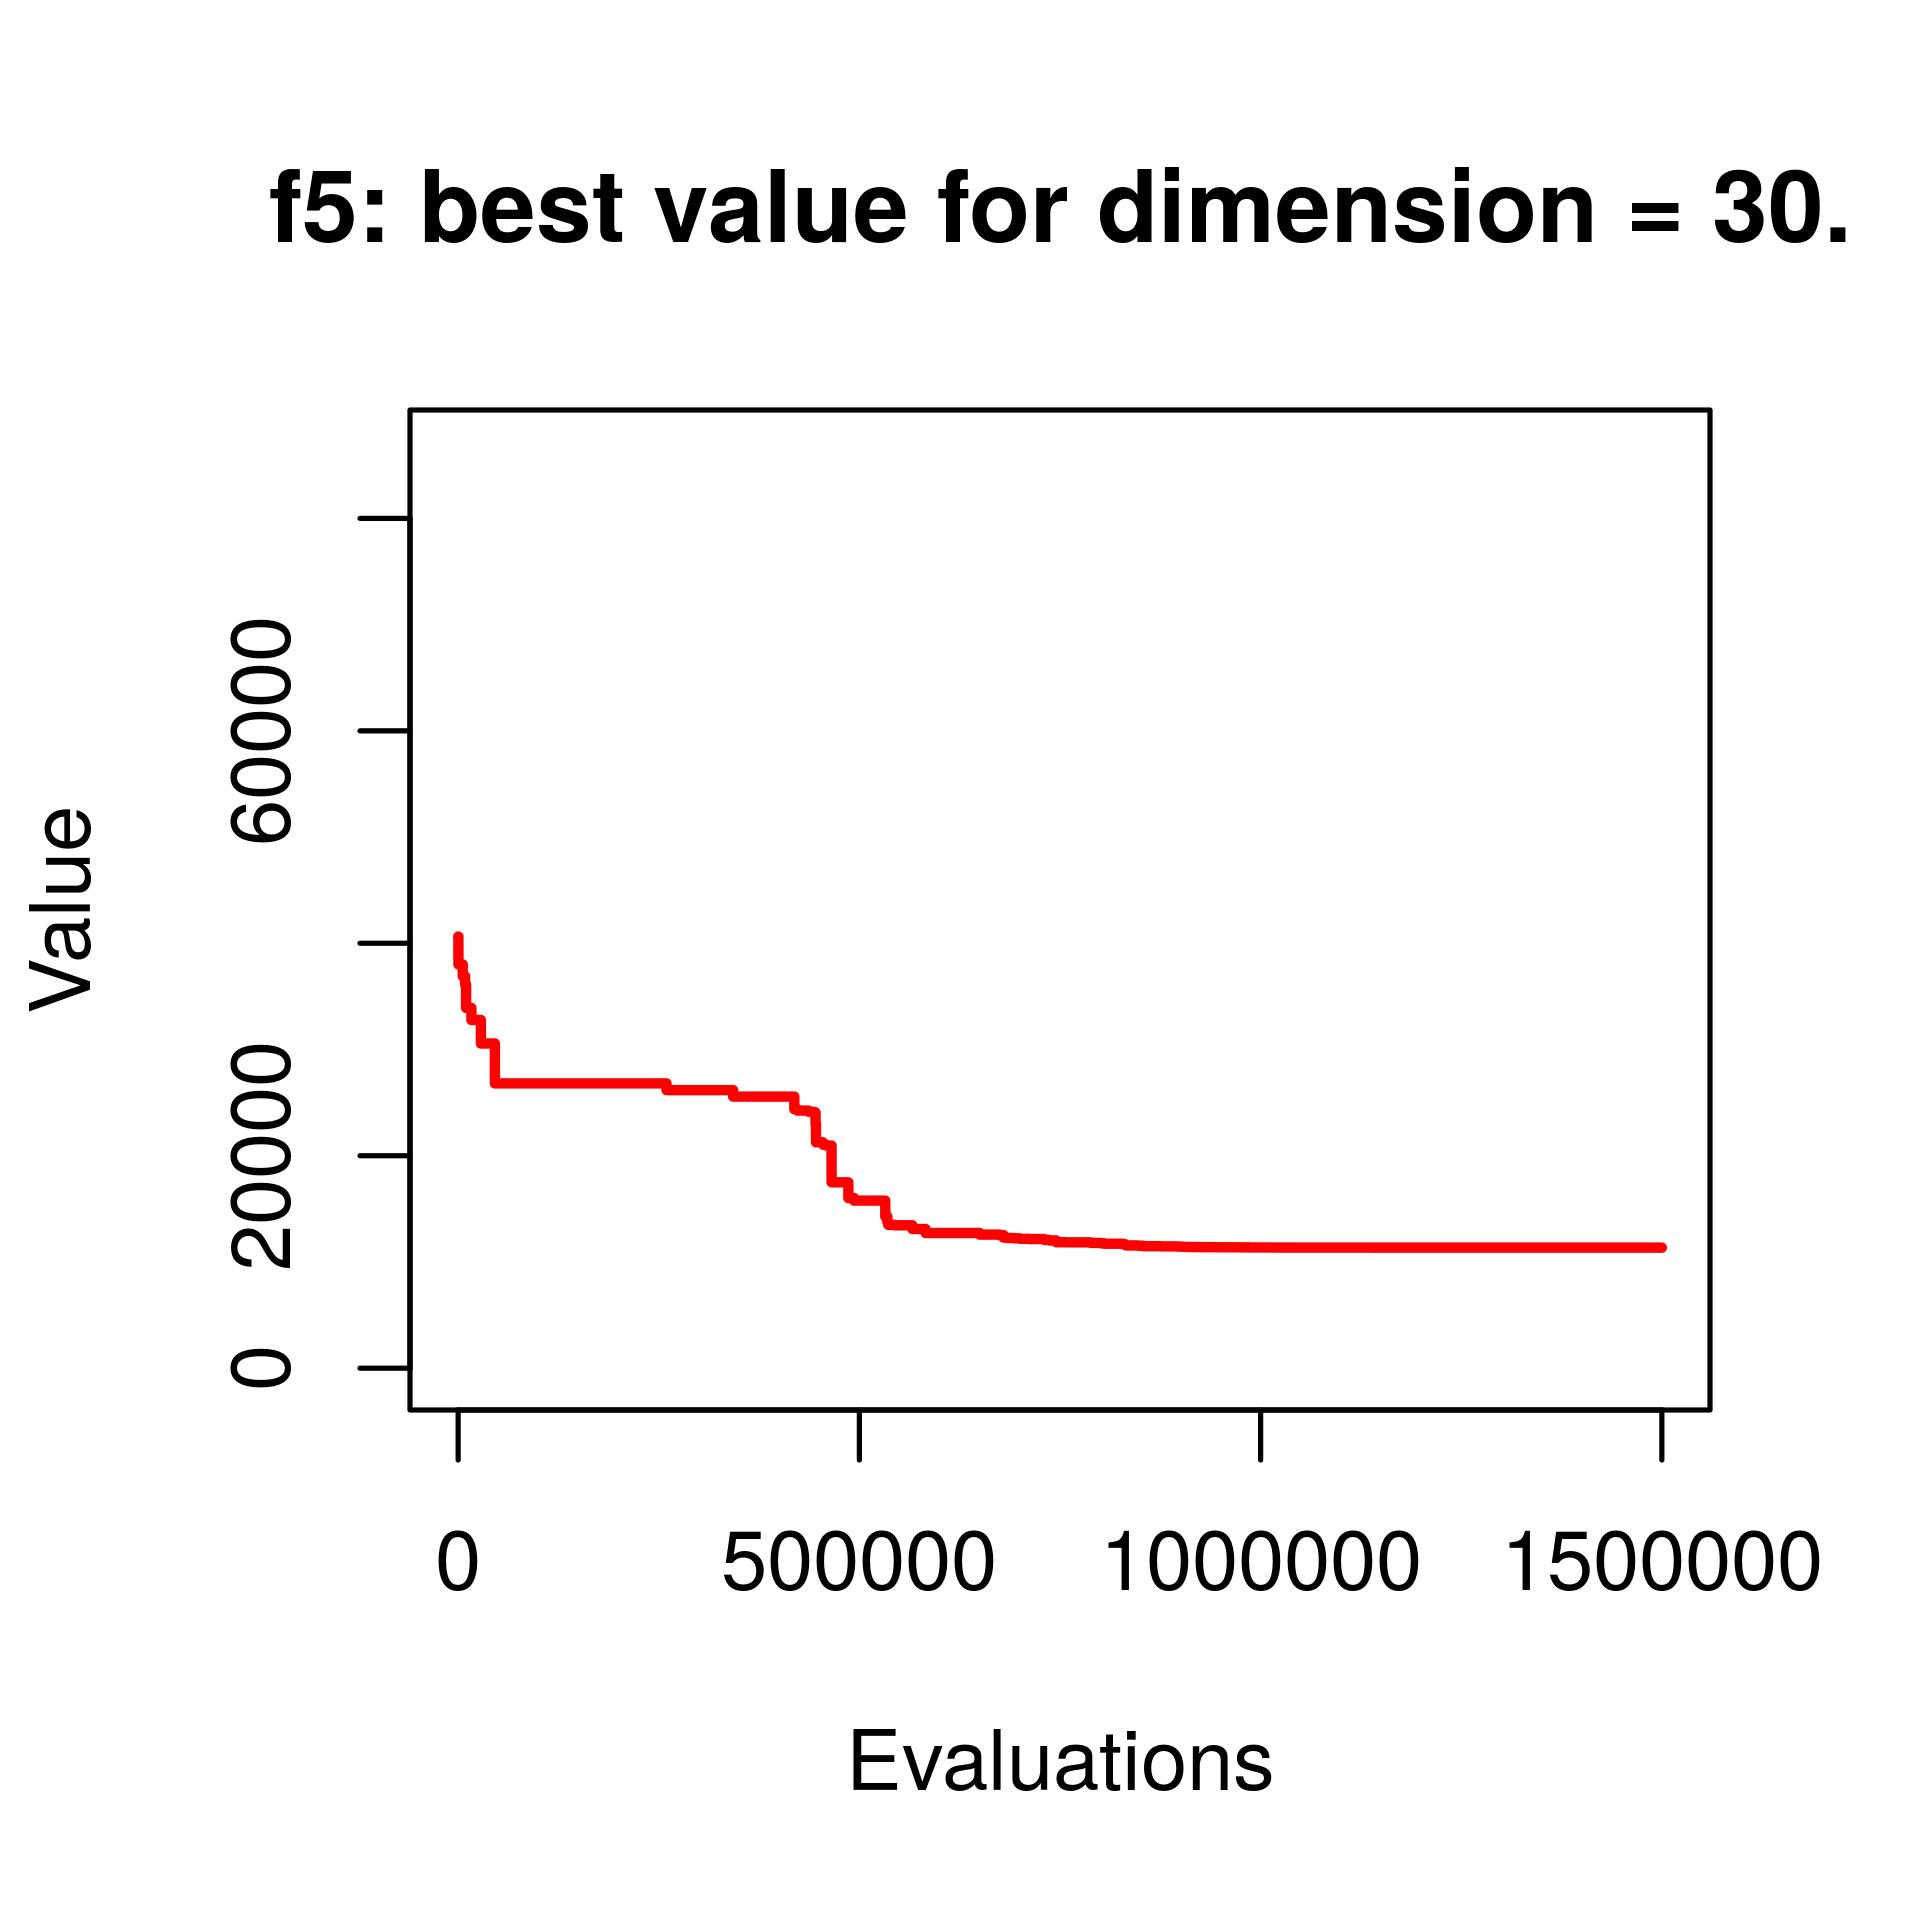
\includegraphics[width=\textwidth]{Imagenes/VS_f5_d30.jpg}
			\caption{Gráfica que representa el mejor valor frente a las evaluaciones para F5 en 30 dimensiones.}
		\end{minipage}
	\end{figure}
	
	\clearpage
	
\section{Mejora del algoritmo: Combinación con Ideology Algorithm}

	\noindent Ante todo agradezco la colaboración de mi compañero Néstor Rodríguez Vico, que ha desarrollado el código de Ideology Algorithm y ha colaborado conmigo en la realización de esta sección.\\

	\noindent Ideology Algorithm es un algoritmo poblacional diseñado para problemas de optimización real que se asemeja a la Evolución Diferencial. Es un algoritmo basado en el comportamiento de los políticos, mantendremos una población de individuos (políticos) agrupadas en subpoblaciones (partidos políticos) que evoluciona según la interacción que se produce entre los individuos de la misma. Las subpoblaciones se mantienen ordenadas según el ajuste que proporcionan los individuos, de esta forma podemos identificar cinco tipos de individuos: el líder, el sublíder, el peor, el segundo peor y el resto de individuos. Dentro de la población llamaremos líder global al mejor individuo de todos. Durante las iteraciones del algoritmo cada individuo genera nuevos individuos de una forma distinta:
	
	\begin{itemize}
		\item El líder, de forma análoga a la vida real, intentará mejorar él sólo (proceso llamado introspección), intentará mejorar fijándose en el sublíder de su partido para intentar seguir siendo el mejor (competición local) e intentará mejorar fijándose líder global para llegar a ser el líder global (competición global).
		\item El peor individuo comprobará si debe seguir en el partido político en el que se encuentra o debe marcharse a otro. Para ello se fijará en cómo de diferente es su forma de pensar (el valor de la solución) con respecto al segundo peor individuo del partido. Si la diferencia es mayor que un umbral, este se marchará a un partido elegido de forma aleatoria.
		\item El resto de individuos intentará mejorar por sí mismo (proceso llamado introspección) e intentarán mejorar fijándose en el líder de su partido (competición local).
	\end{itemize}
	
	
	\noindent La combinación de los algoritmos de Búsqueda por Vórtices e Ideology Algorithm consiste en emplear la búsqueda por vórtices como mejora local para los individuos de la población, es decir, los políticos, obteniendo como resultado un algoritmo memético. Puesto que, para el problema que nos atañe, los políticos no son mas que puntos en el espacio, podemos dar el punto en el espacio asociado al político como centro inicial para la búsqueda por vórtices, de esta forma lanzamos una búsqueda por trayectorias simples en el área del espacio que rodea al político. Los resultados obtenidos con la combinación de estos algoritmos son los siguientes:\\
	
	\begin{table}[h]
		\centering
		\setlength{\arrayrulewidth}{1mm}
		\setlength{\tabcolsep}{10pt}
		\renewcommand{\arraystretch}{1.1}
		
		\rowcolors{2}{gray!25}{white}
		\begin{tabular}{ >{\centering\arraybackslash}m{1.15cm}  >{\centering\arraybackslash}m{1.2cm}  >{\centering\arraybackslash}m{1.2cm}   >{\centering\arraybackslash}m{1.4cm}  >{\centering\arraybackslash}m{1.15cm}  >{\centering\arraybackslash}m{1.2cm}  >{\centering\arraybackslash}m{1.2cm}   >{\centering\arraybackslash}m{1.4cm}  }
			\hline
			\rowcolor{black}
			\multicolumn{8}{c}{\bf \color{white}{Algoritmo Combinado (Dimensión 10)}}\\
			\hline
			\rowcolor{gray!50}
			\textbf{Función} & \textbf{Valor} & \textbf{Optimo} & \textbf{Desv.} & \textbf{Función} & \textbf{Valor} & \textbf{Optimo} & \textbf{Desv.} \\
			F1 & -449.9 & -450.0 & 0.0221 & F10 & -321.1 & -330.0 & 2.72  \\
			F2 & -449.1 & -450.0 & 0.188 & F11 & 91.95 & 90.0 & 2.172   \\
			F5 & 81.12 & -310.0 & 126.169 & F13 & -129.3 & -130.0 & 0.53 \\
			F6 & 399.798 & 390.0 & 2.5127 & F14 & -297.87 & -300.0 & 0.71 \\
			F8 & -119.97 & -140.0 & 14.3 & F17 & 163.946 & 120.0 & 36.62 \\
			F9 & -324.86 & -330.0 & 1.556 & F24 & 460.04 & 260.0 & 76.93 \\
			
			\hline
			
		\end{tabular}
		
	\end{table}
	
	\clearpage
	
	\noindent A continuación se muestran los resultados obtenidos por el algoritmo memético para dimensión 30, a excepción de las dos últimas funciones, de las que no se han obtenido resultados por falta de tiempo.\\
	
	\begin{table}[h]
		\centering
		\setlength{\arrayrulewidth}{1mm}
		\setlength{\tabcolsep}{10pt}
		\renewcommand{\arraystretch}{1.1}
		
		\rowcolors{2}{gray!25}{white}
		\begin{tabular}{ >{\centering\arraybackslash}m{1.15cm}  >{\centering\arraybackslash}m{1.2cm}  >{\centering\arraybackslash}m{1.2cm}   >{\centering\arraybackslash}m{1.4cm}  >{\centering\arraybackslash}m{1.15cm}  >{\centering\arraybackslash}m{1.2cm}  >{\centering\arraybackslash}m{1.2cm}   >{\centering\arraybackslash}m{1.4cm}  }
			\hline
			\rowcolor{black}
			\multicolumn{8}{c}{\bf \color{white}{Algoritmo Combinado (Dimensión 30)}}\\
			\hline
			\rowcolor{gray!50}
			\textbf{Función} & \textbf{Valor} & \textbf{Optimo} & \textbf{Desv.} & \textbf{Función} & \textbf{Valor} & \textbf{Optimo} & \textbf{Desv.} \\
			F1 & 82.87 & -450.0 & 118.41 & F10 & -148.32 & -330.0 & 55.1  \\
			F2 & 2256.158 & -450.0 & 601.37 & F11 & 114.37 & 90.0 & 27.07 \\
			F5 & 6536.26 & -310.0 & 2208.5 & F13 & -111.19 & -130.0 & 14.472 \\
			F6 & 1675756 & 390.0 & 429581 & F14 & -288.1 & -300.0 & 3.9674 \\
			F8 & -119.67 & -140.0 & 14.52 & F17 & X & X & X \\
			F9 & -164 & -330.0 & 50.3 & F24 & X & X & X \\
			
			\hline
			
		\end{tabular}
		
	\end{table}
	
	\noindent A la vista de los resultados podemos decir que, claramente la combinación de estos dos algoritmos no parece ser la ideal para resolver algunos de los problemas de optimización que la búsqueda por vórtices es capaz de resolver, sin embargo, y aunque estos casos sean la minoría, la combinación parece presentar mejora, por ejemplo, para las funciones F9 y F10.\\
	
	\noindent Para obtener una mejor idea del comportamiento de este algoritmo, de igual forma que hacíamos con la búsqueda por vórtices, podemos representar el mejor valor obtenido frente a las evaluaciones realizadas:
	
	\begin{figure}[!h]
		\centering
		\begin{minipage}[b]{0.4\textwidth}
			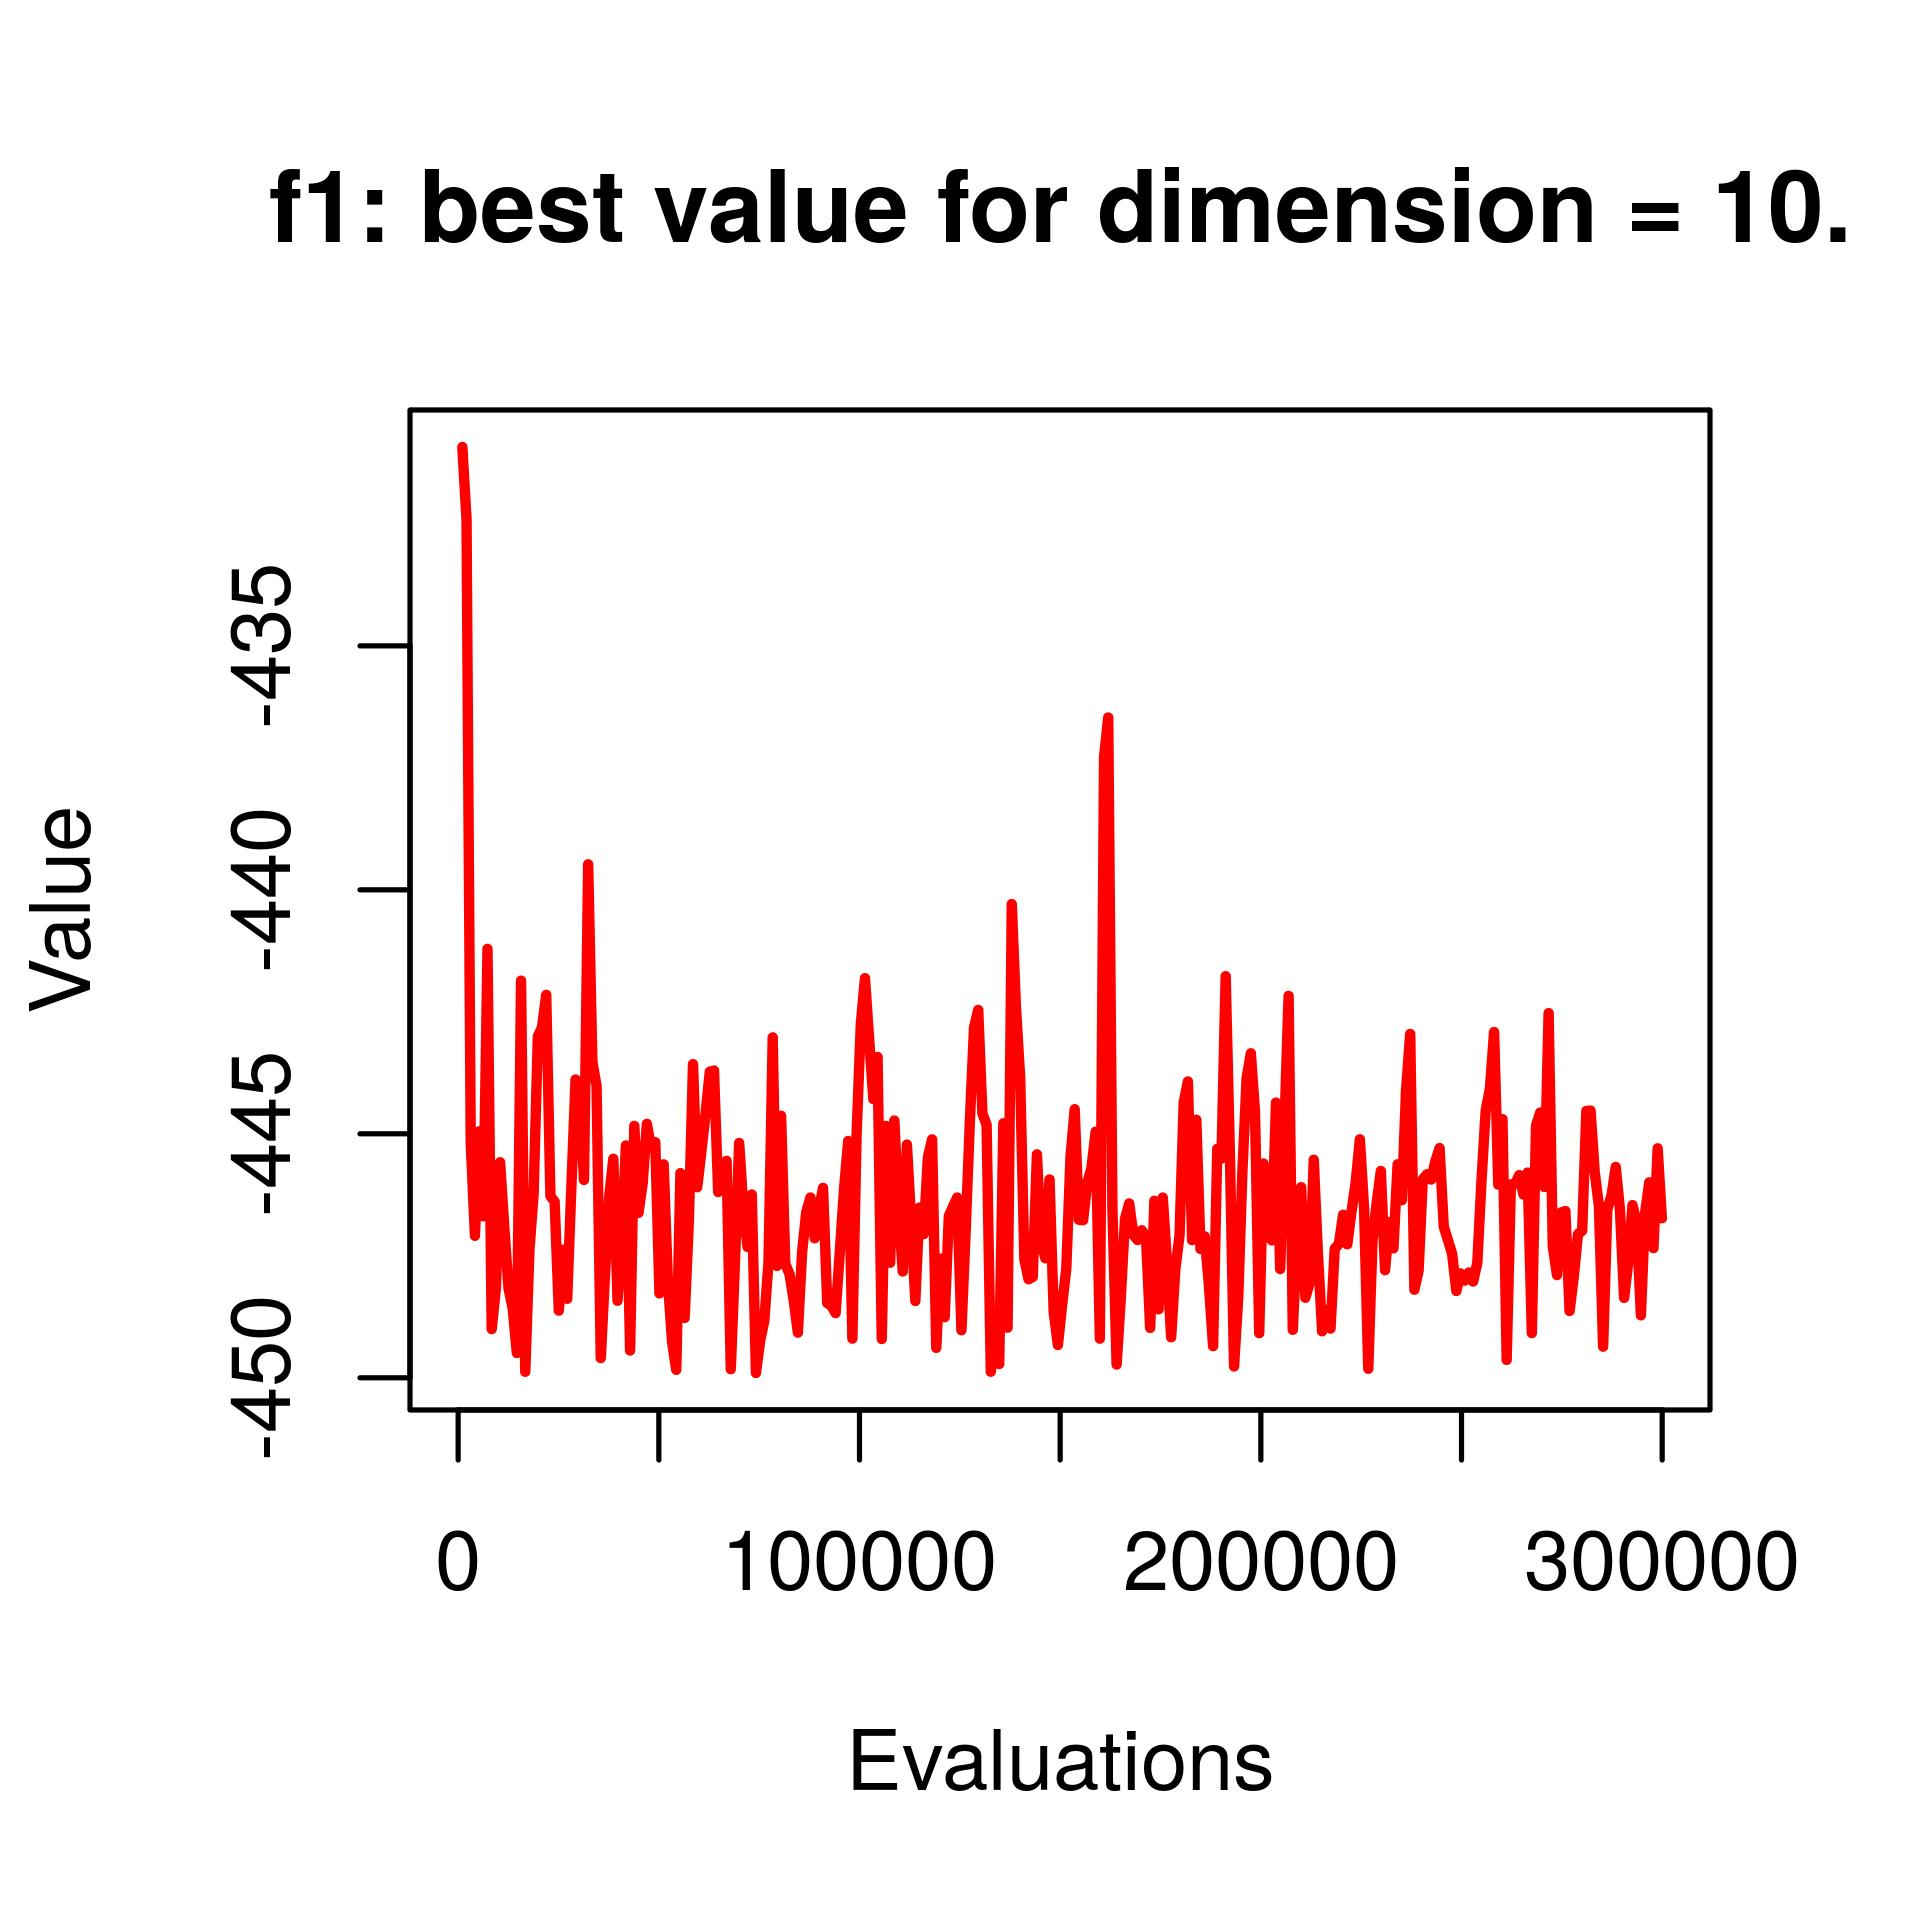
\includegraphics[width=\textwidth]{Imagenes/MM_f1_d10.jpg}
			\caption{Gráfica que representa el mejor valor frente a las evaluaciones para F1 en 30 dimensiones.}
		\end{minipage}
		\hfill
		\begin{minipage}[b]{0.4\textwidth}
			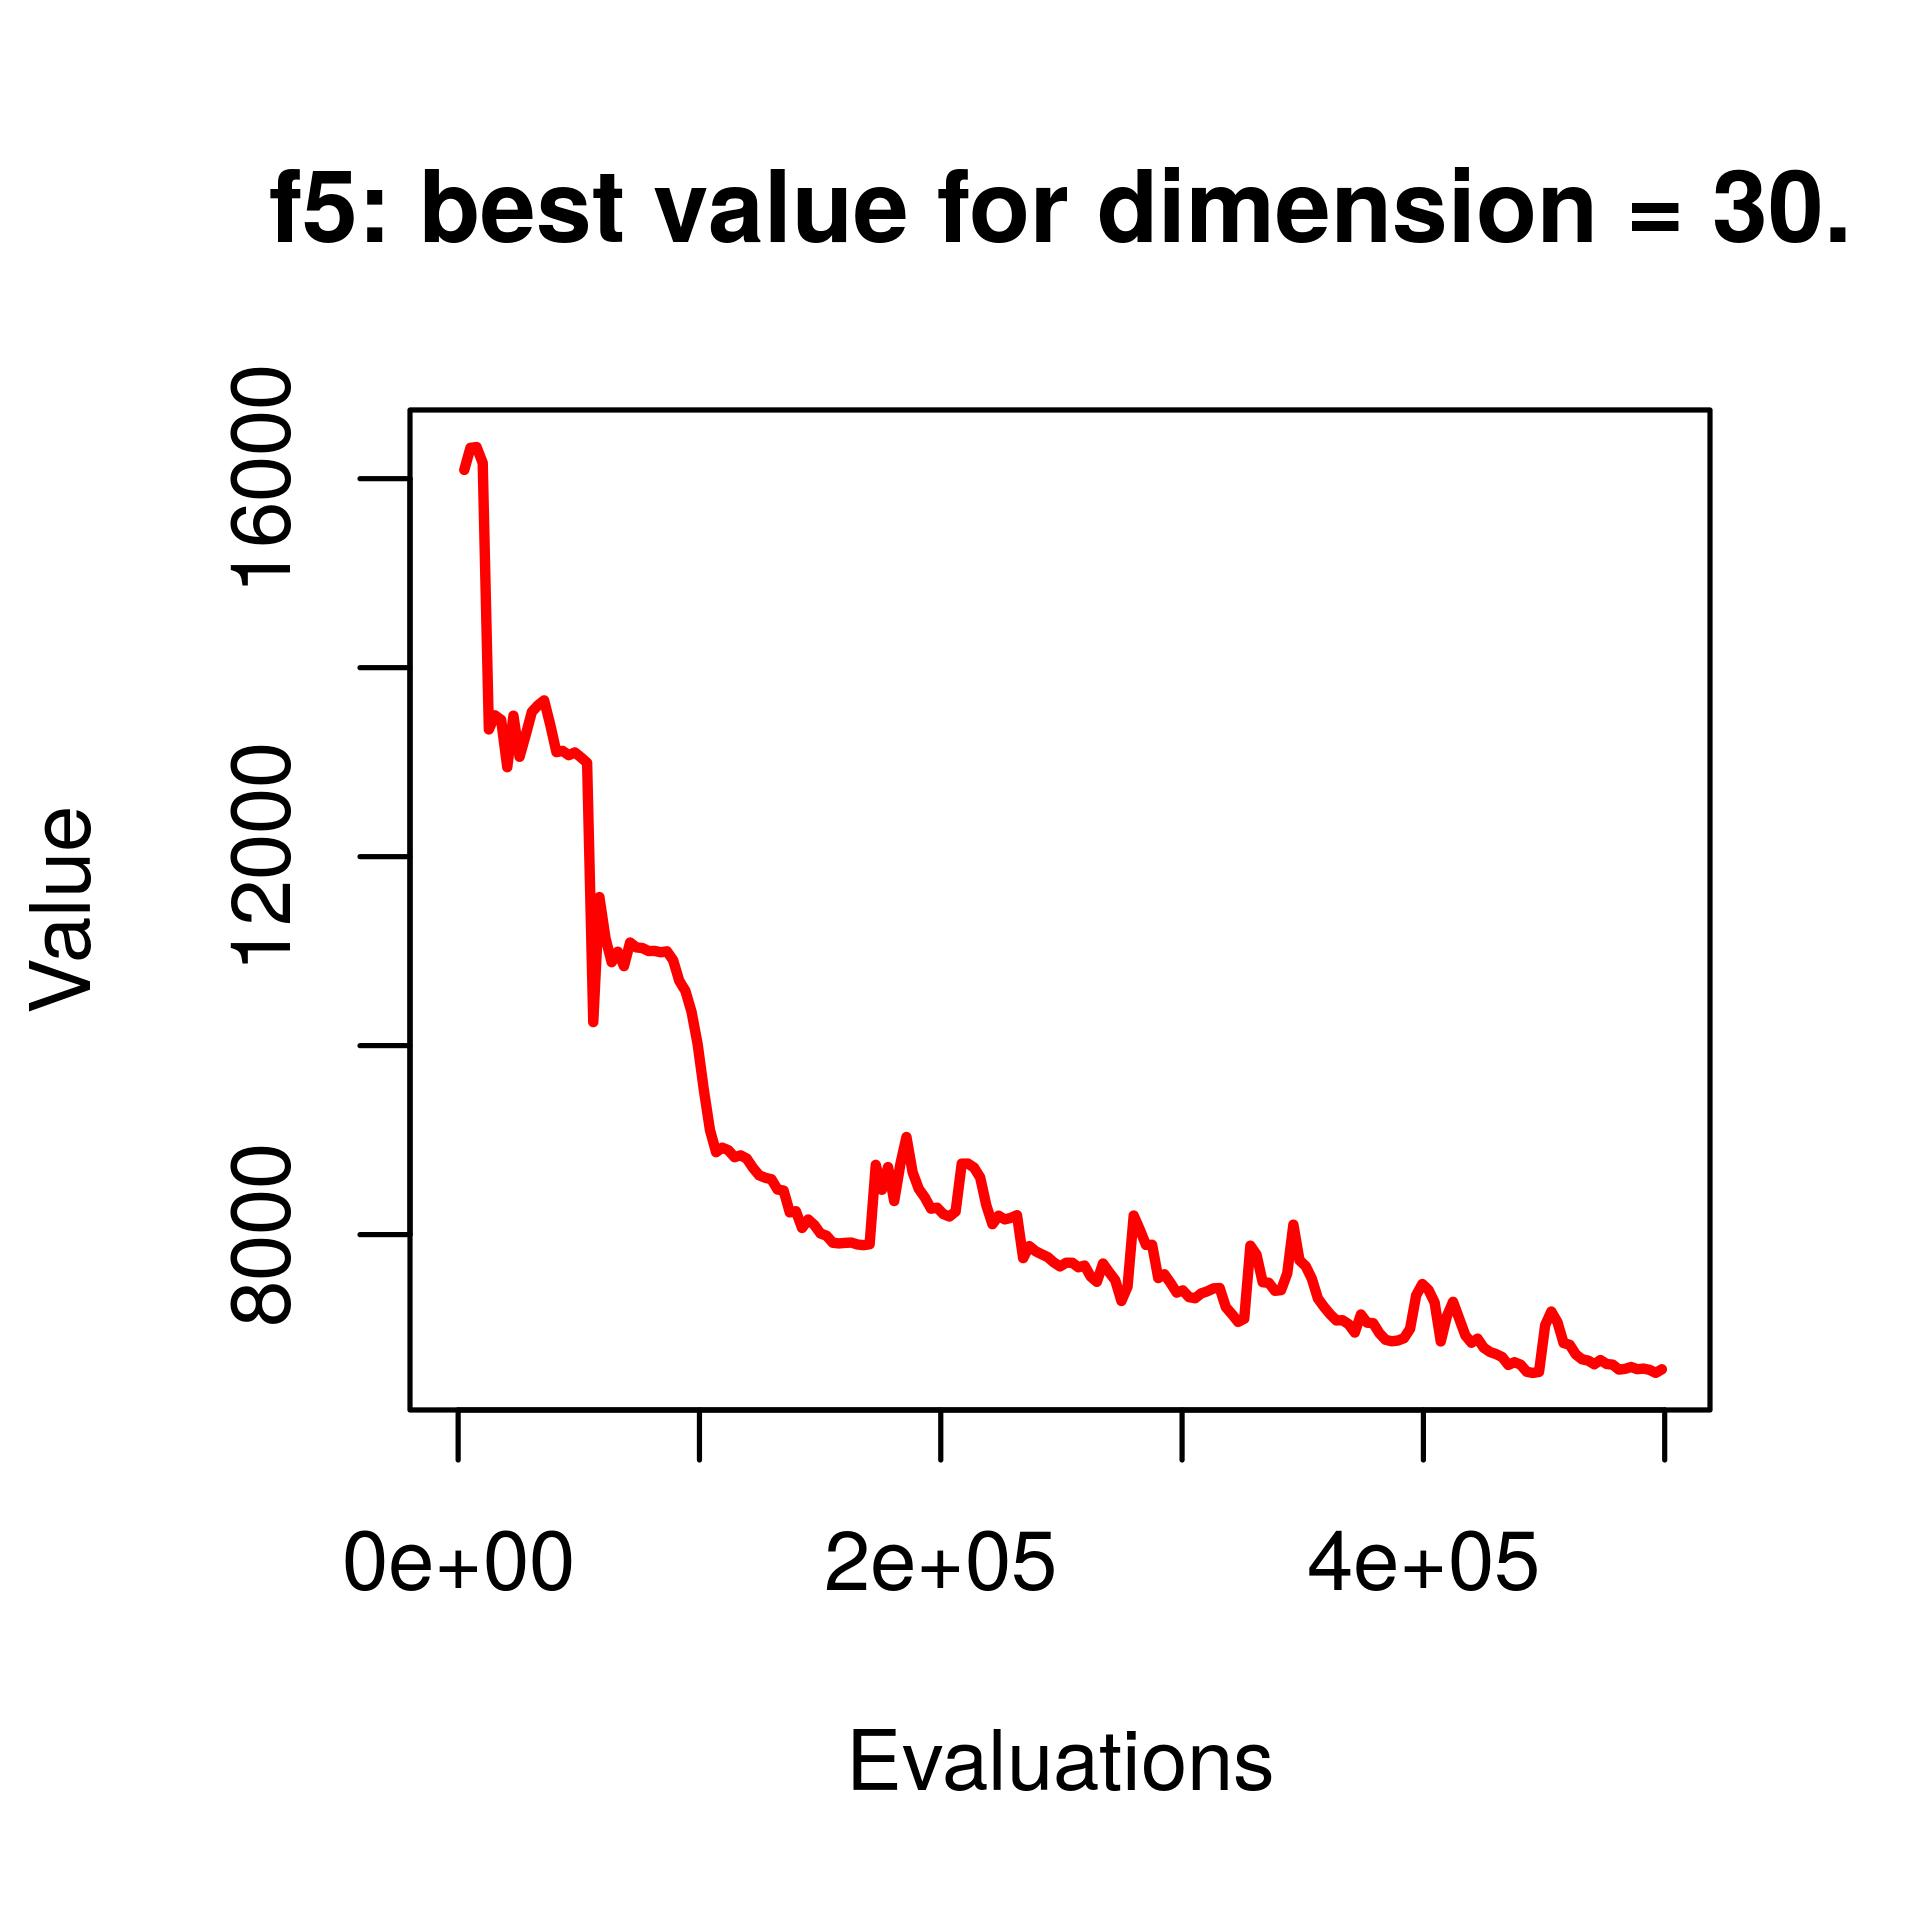
\includegraphics[width=\textwidth]{Imagenes/MM_f5_d10.jpg}
			\caption{Gráfica que representa el mejor valor frente a las evaluaciones para F5 en 30 dimensiones.}
		\end{minipage}
	\end{figure}
	
	\noindent Como era de esperar, el mejor valor obtenido disminuye con el paso de las iteraciones, la diferencia más notable que encontramos en estas gráficas respecto a las de la búsqueda por vórtices es que, al contrario de lo que sucedía en esta última, Ideology Algorithm es capaz de explorar soluciones peores a la actual en cada iteración. Además cabe destacar que el comportamiento del algoritmo depende en gran medida de la función considerada para la optimización, es por ello que vemos grandes fluctuaciones en el mejor valor en la función 1, al contrario de lo que sucede en la función 5.
	
\clearpage
	
\section{Mejoras consideradas para el algoritmo memético}

	\noindent Una de las mejoras inmediatas que podemos considerar para un algoritmo memético es el reinicio de la población cuando detectamos que esta converge a un valor. Por tanto, podemos aplicar esta técnica al algoritmo desarrollado en la sección anterior. Sin embargo, tras la experimentación, la conclusión es que, dadas las características del algoritmo, así como de las funciones a optimizar, no es posible establecer un patrón para la identificación del umbral del reinicio de la población; de esta forma, los resultados obtenidos son, en general, peores que los obtenidos con el algoritmo memético básico.\\
	
	\noindent Dadas las características del algoritmo consideramos como reinicio de la población la generación de nuevos individuos aleatorios, en concreto, 150 de ellos, y su posterior agrupación en partidos del mismo tamaño, a saber, 30. Teniendo esto en consideración, planteamos las siguientes técnicas para detección de momentos de reinicio:
	
	\subsection{Reinicio por diferencia de tamaño de partidos}
	
		\noindent Esta técnica consiste en reiniciar la población cuando se detecta que el partido mayoritario es un tanto por ciento mayor que el minoritario, es decir, consideramos que la población converge cuando la mayoría de individuos se encuentran en el partido mayoritario, lo que se traduce en que la mayoría de individuos sean similares.\\
		
		\noindent Los resultados obtenidos con esta técnica son, en el mejor de los casos iguales a los obtenidos sin ella. Podemos obtener una representación visual de lo que le sucede a la población durante el proceso de búsqueda representando los tamaños de los partidos mayoritarios y minoritarios frente al número de evaluaciones:
		
		\begin{figure}[!h]
			\centering
			\begin{minipage}[b]{0.4\textwidth}
				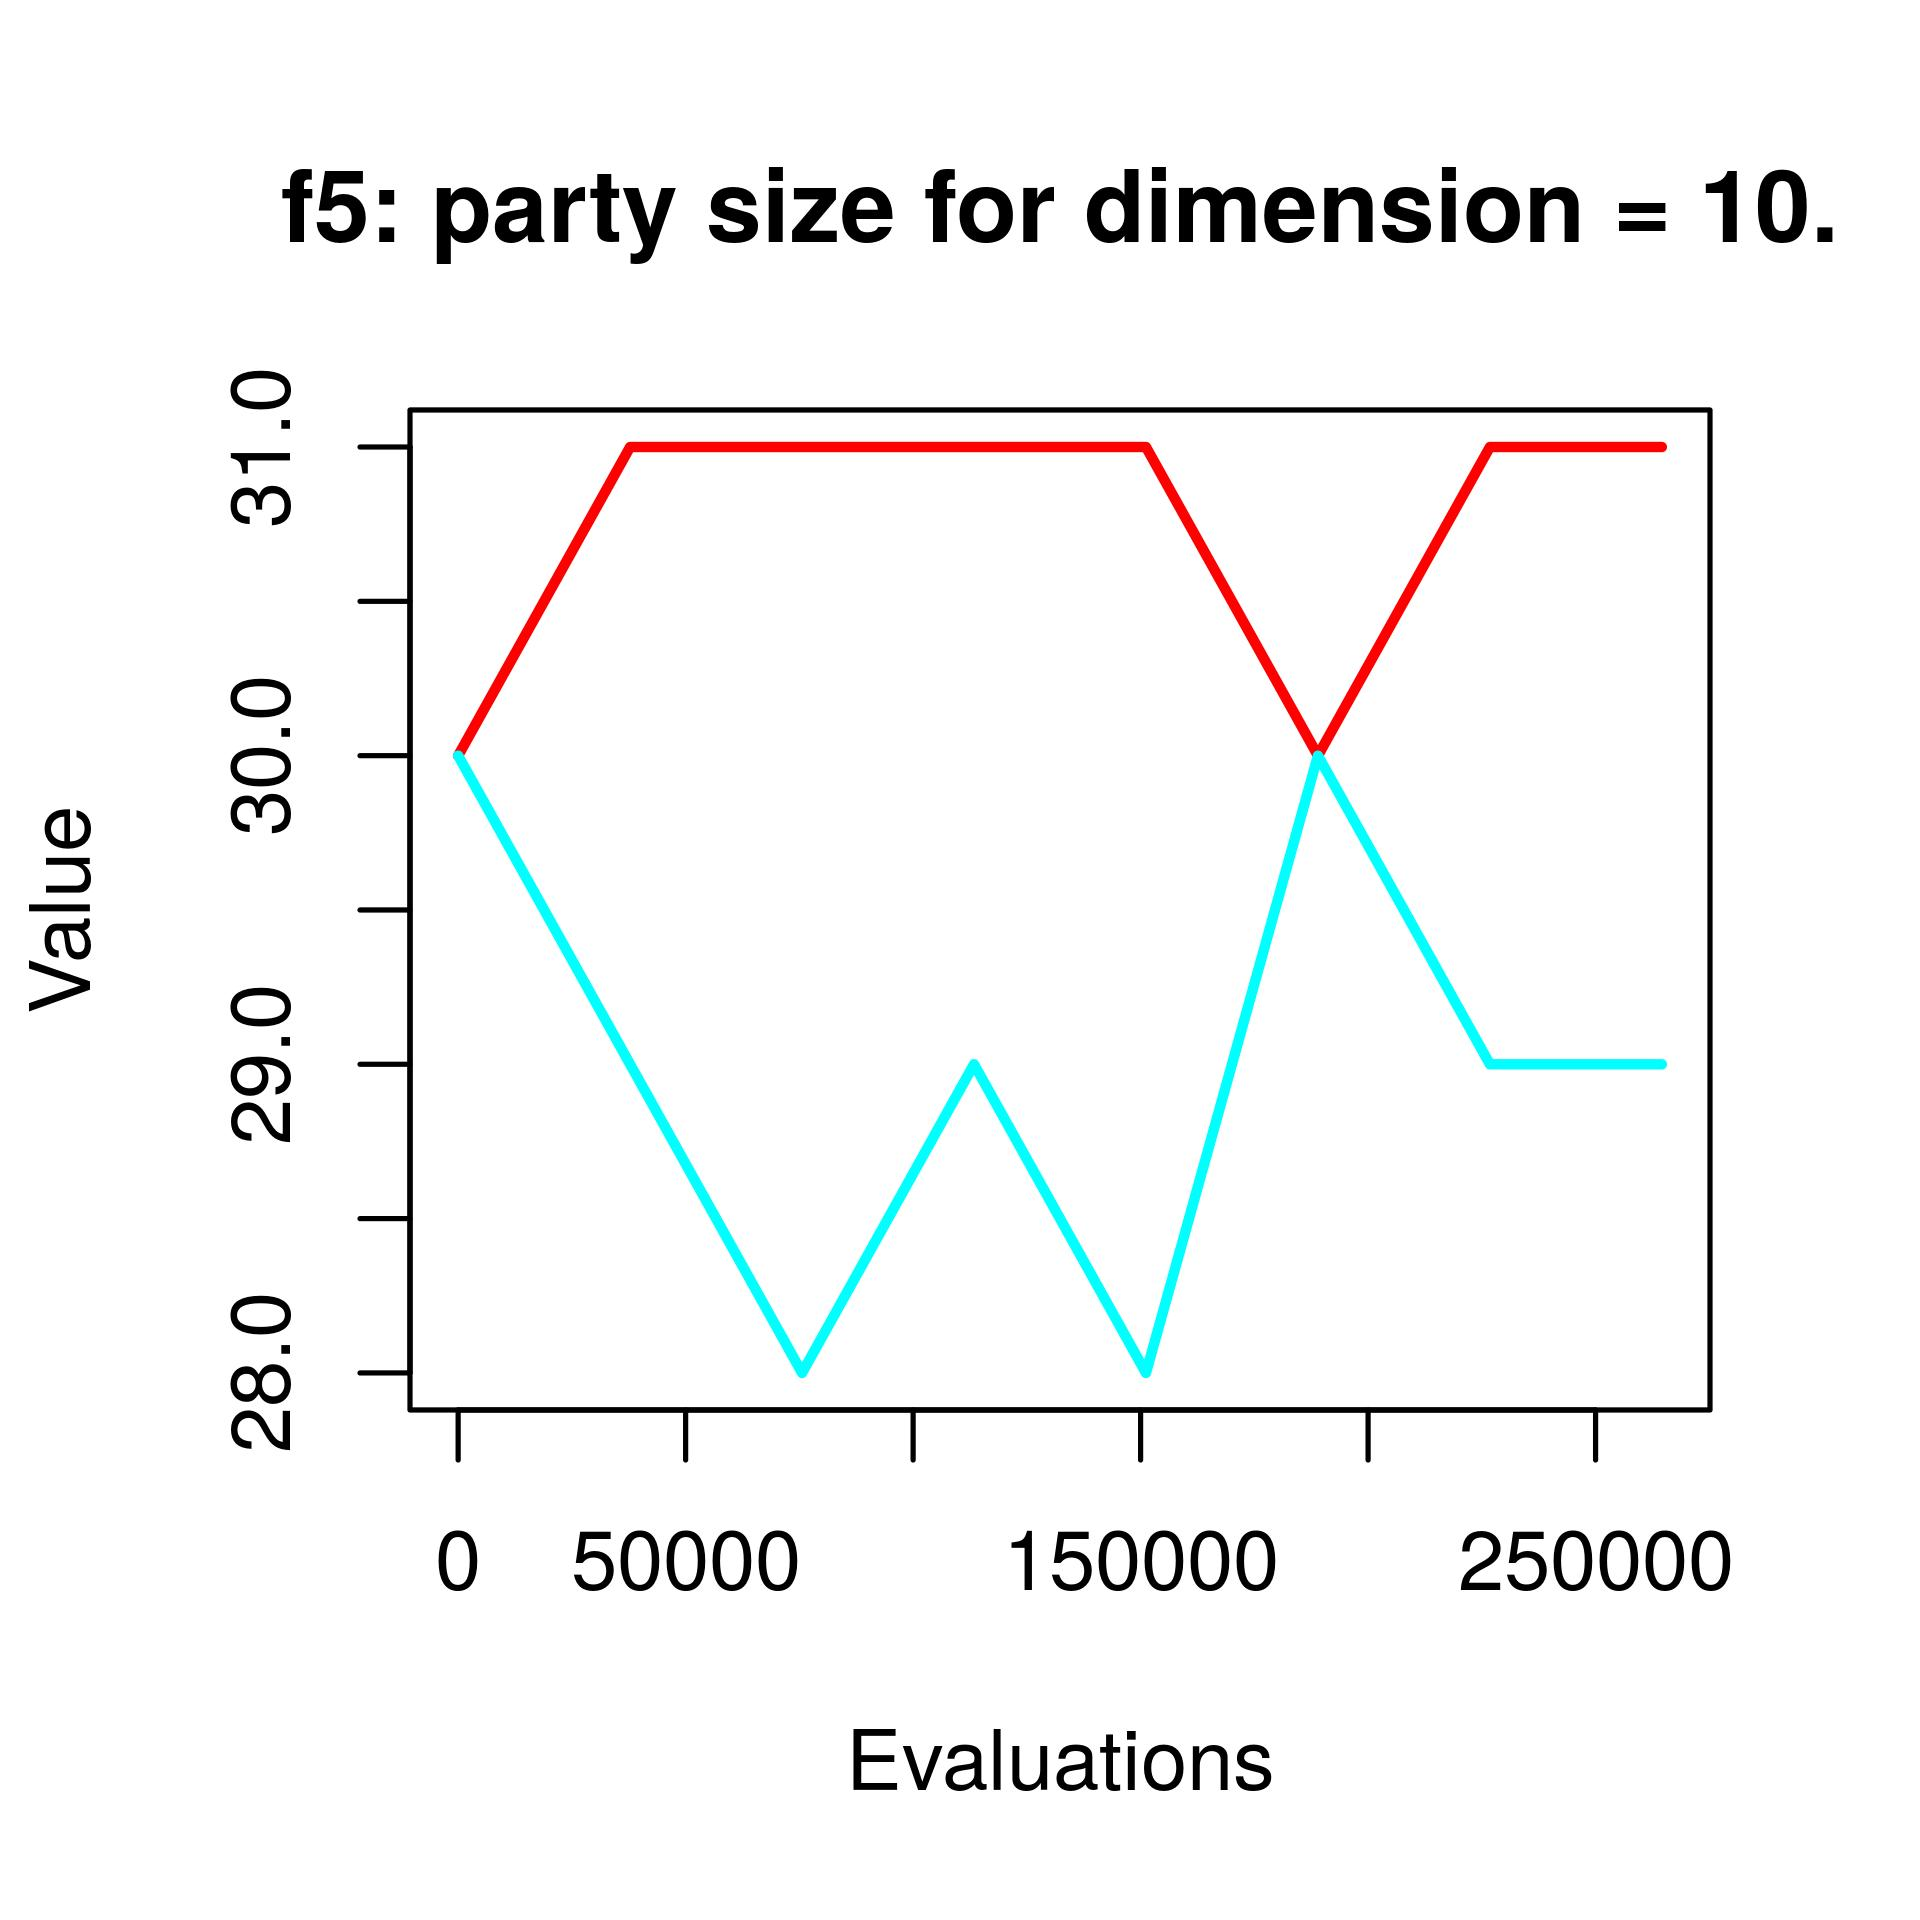
\includegraphics[width=\textwidth]{Imagenes/f5_percentage_10.jpg}
				\caption{Gráfica que representa el número de individuos del partido mayor y menor para F6.}
			\end{minipage}
			\hfill
			\begin{minipage}[b]{0.4\textwidth}
				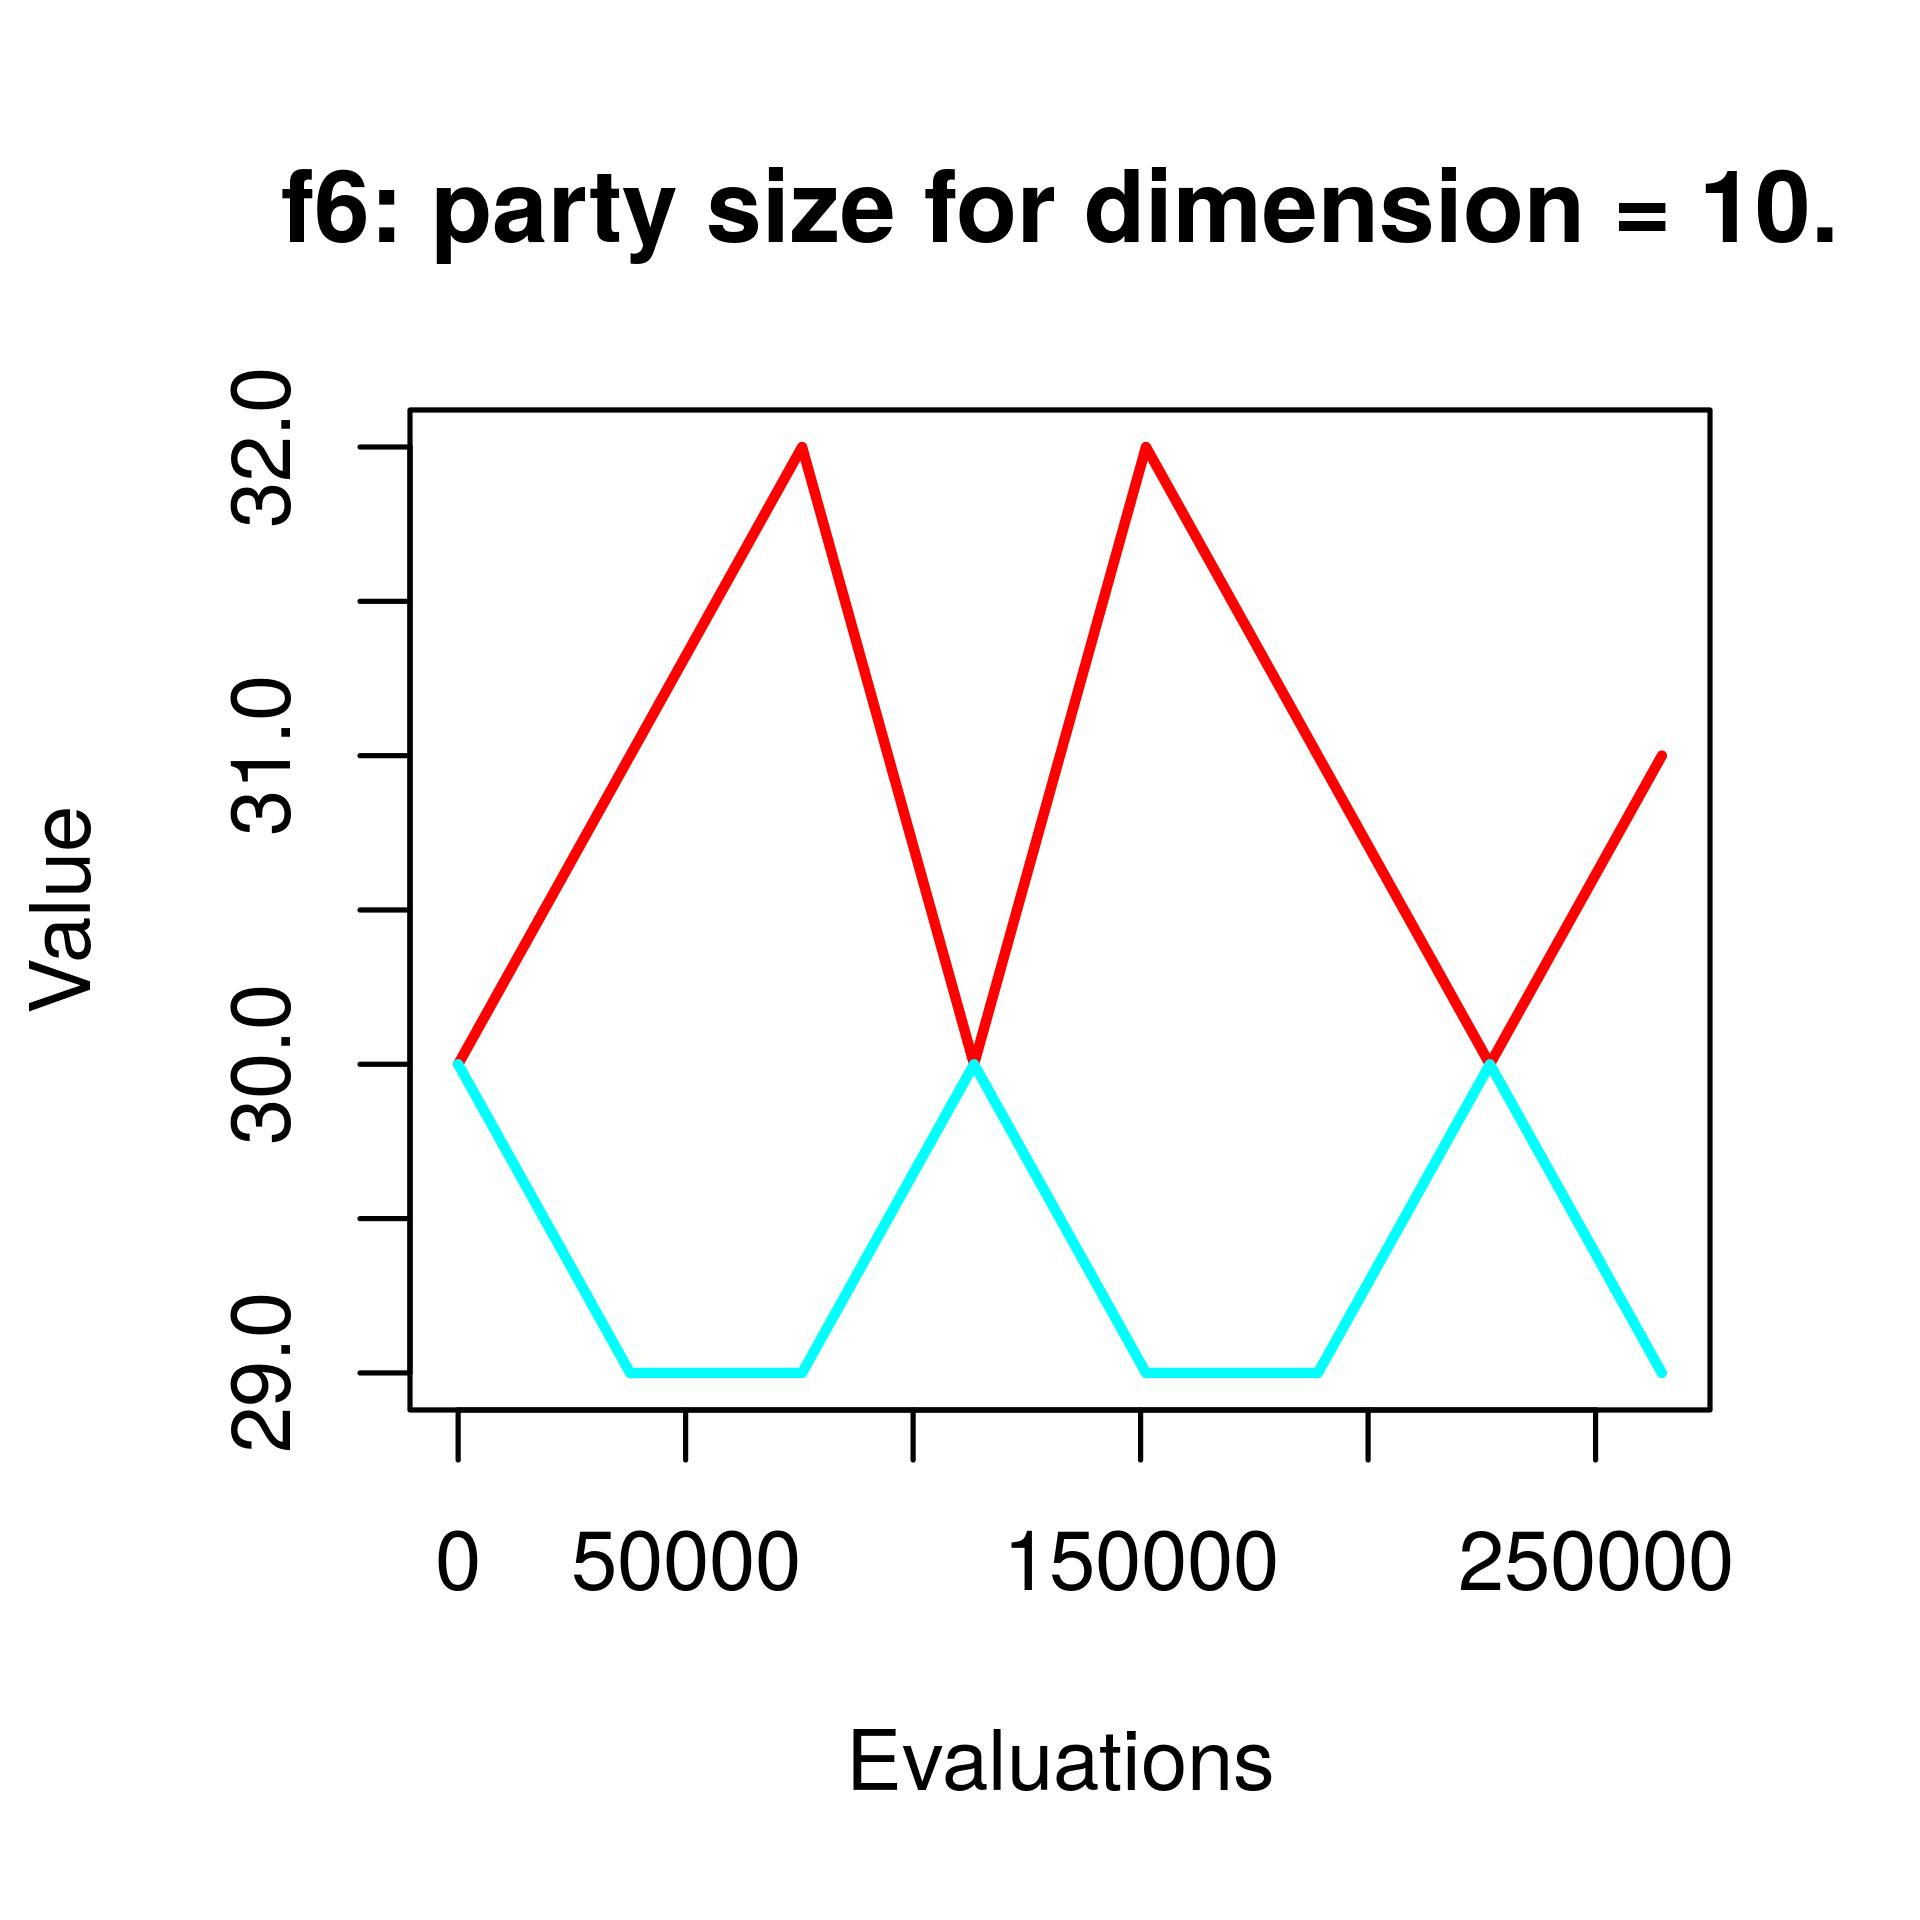
\includegraphics[width=\textwidth]{Imagenes/f6_percentage_10.jpg}
				\caption{Gráfica que representa el número de individuos del partido mayor y menor para FX.}
			\end{minipage}
		\end{figure}
		
		\noindent Encontramos dos casos generales opuestos, el caso en el que la población se reinicia varias veces, y el caso en el que se reinicia una única vez.
	
	
\clearpage

	\subsection{Reinicio por estabilización del mejor individuo}
	
		\noindent Esta técnica consiste en reiniciar la población cuando se detecta que el mejor individuo se estanca, es decir, no mejora con el paso de las iteraciones, lo que se traduce en que el proceso ha pasado de ser de exploración a ser de explotación.\\
		
		\noindent De igual forma que sucedía en el caso anterior, esta técnica no mejora el comportamiento del algoritmo, representaremos gráficamente lo que le sucede a la población durante el proceso de búsqueda:
		
		\begin{figure}[!h]
			\centering
			\begin{minipage}[b]{0.4\textwidth}
				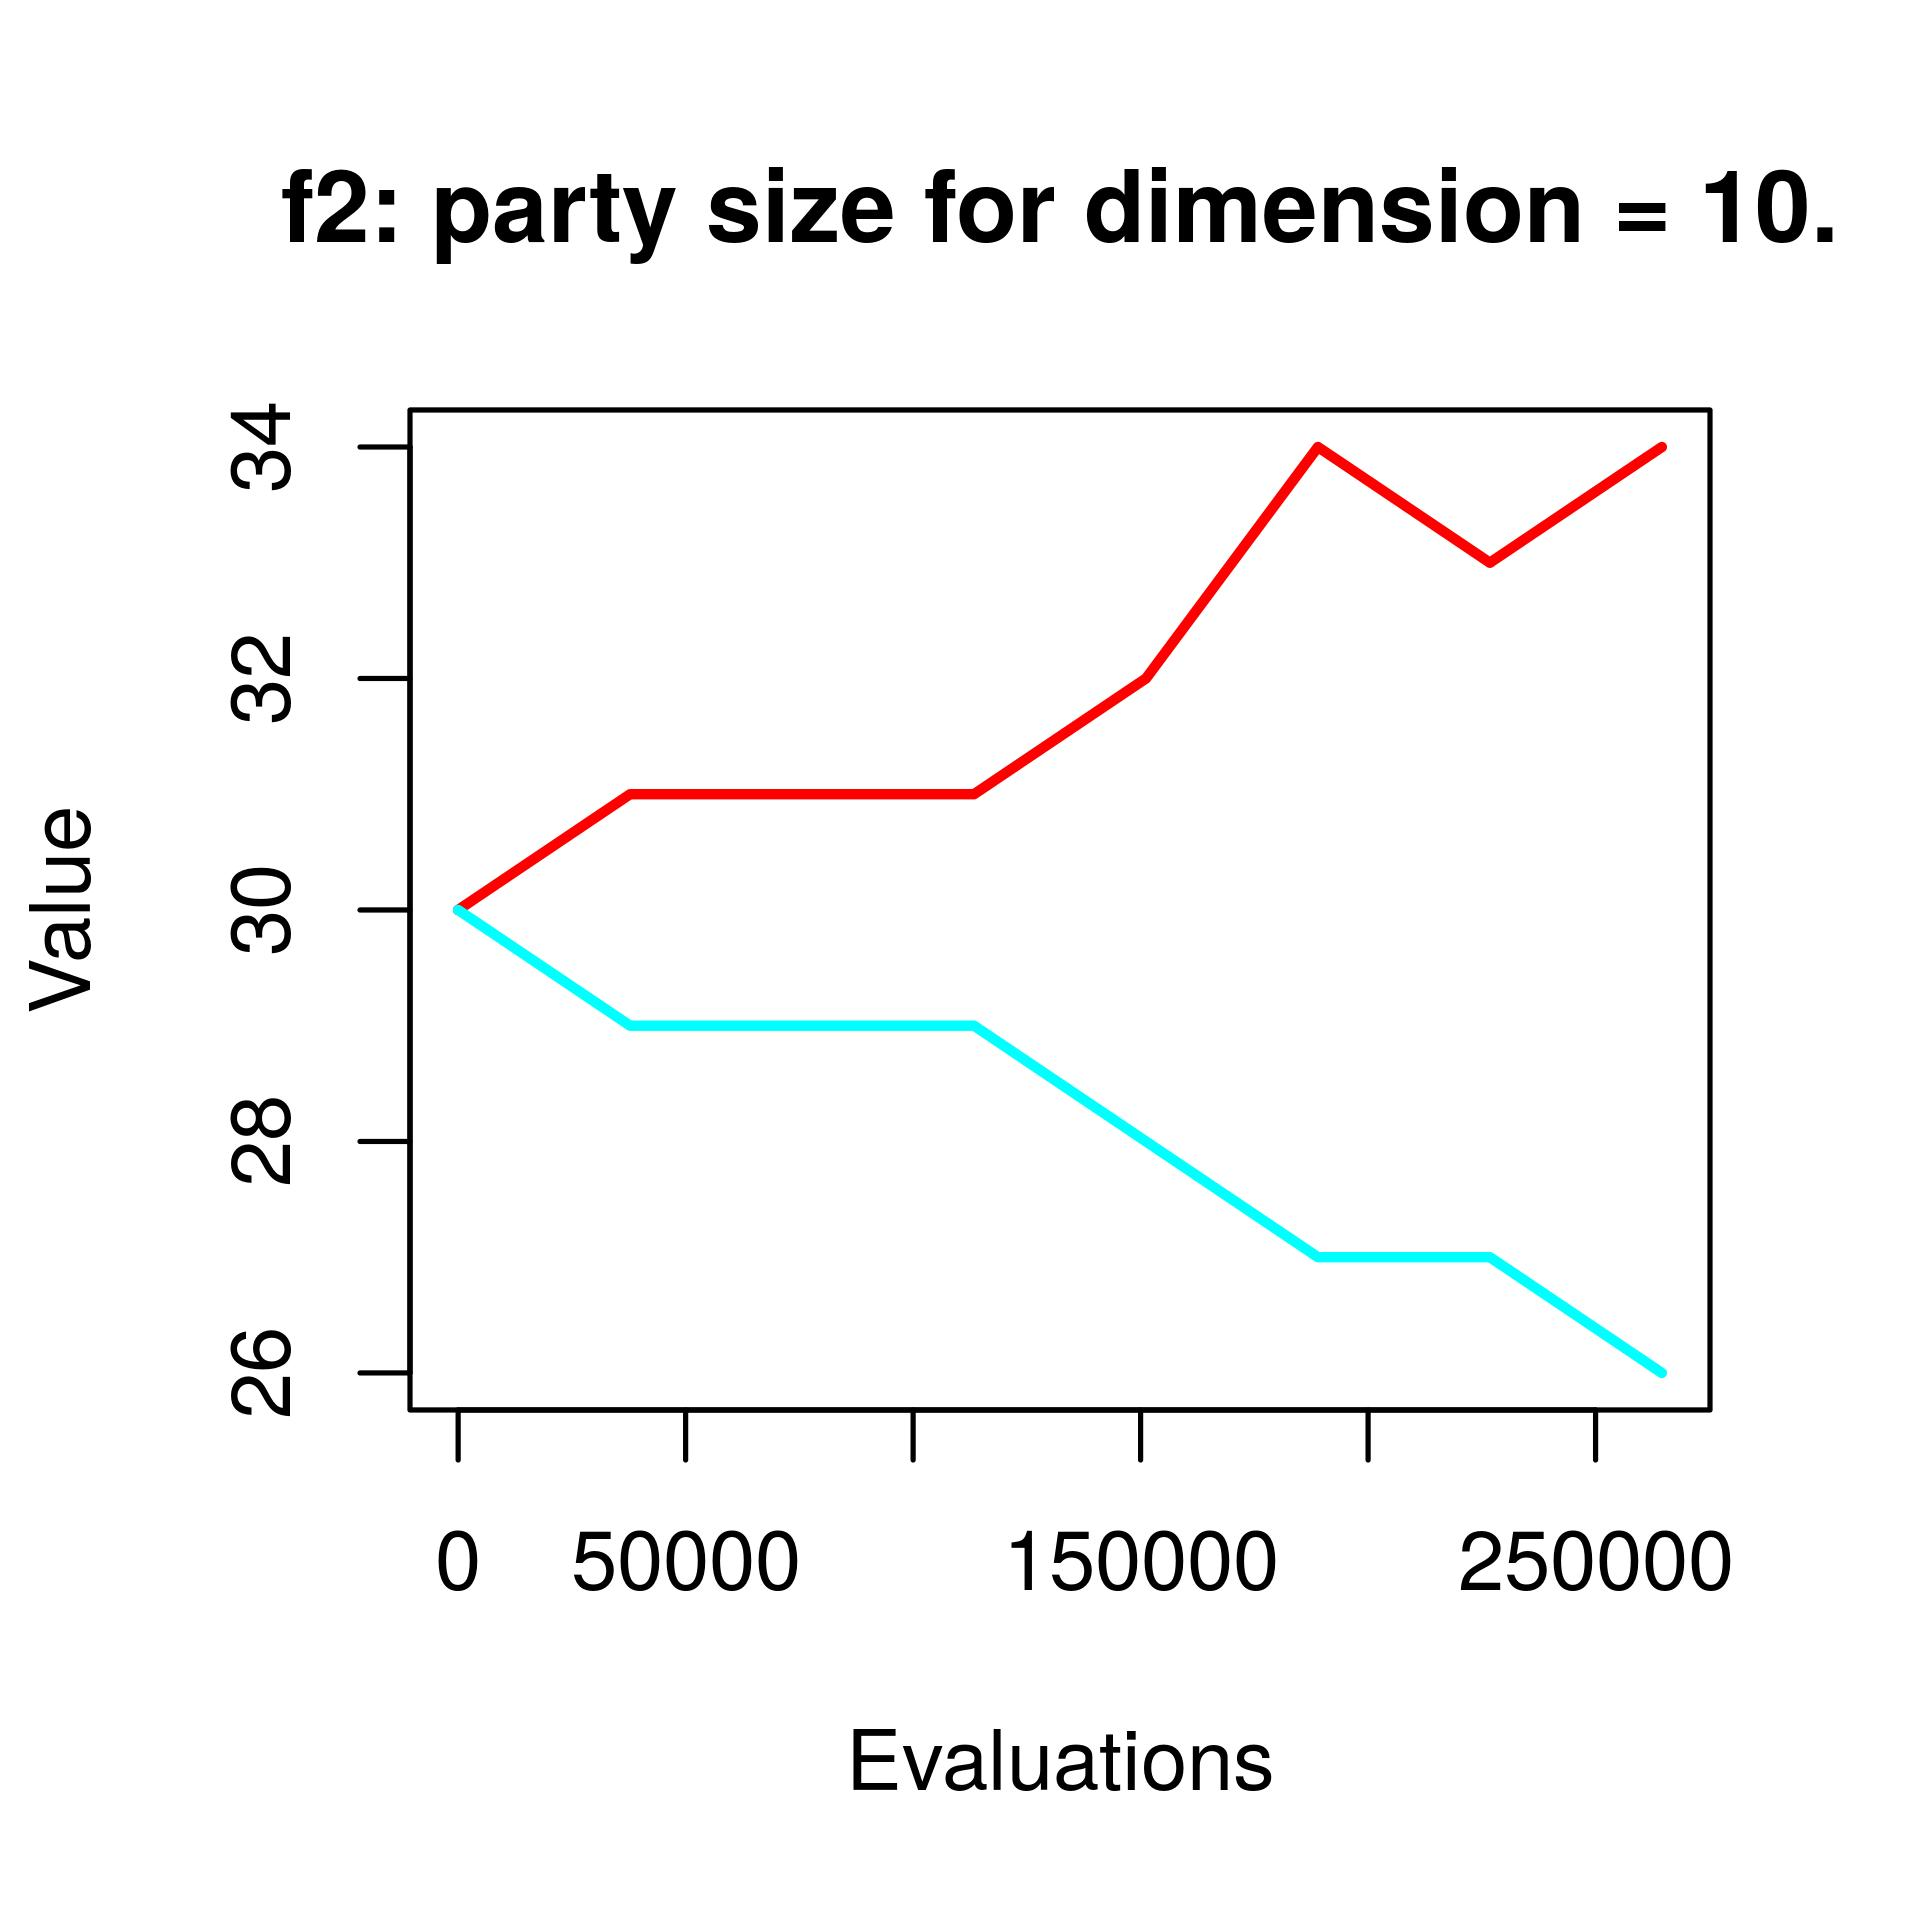
\includegraphics[width=\textwidth]{Imagenes/f2_convergence_10.jpg}
				\caption{Gráfica que representa el número de individuos del partido mayor y menor para F2.}
			\end{minipage}
			\hfill
			\begin{minipage}[b]{0.4\textwidth}
				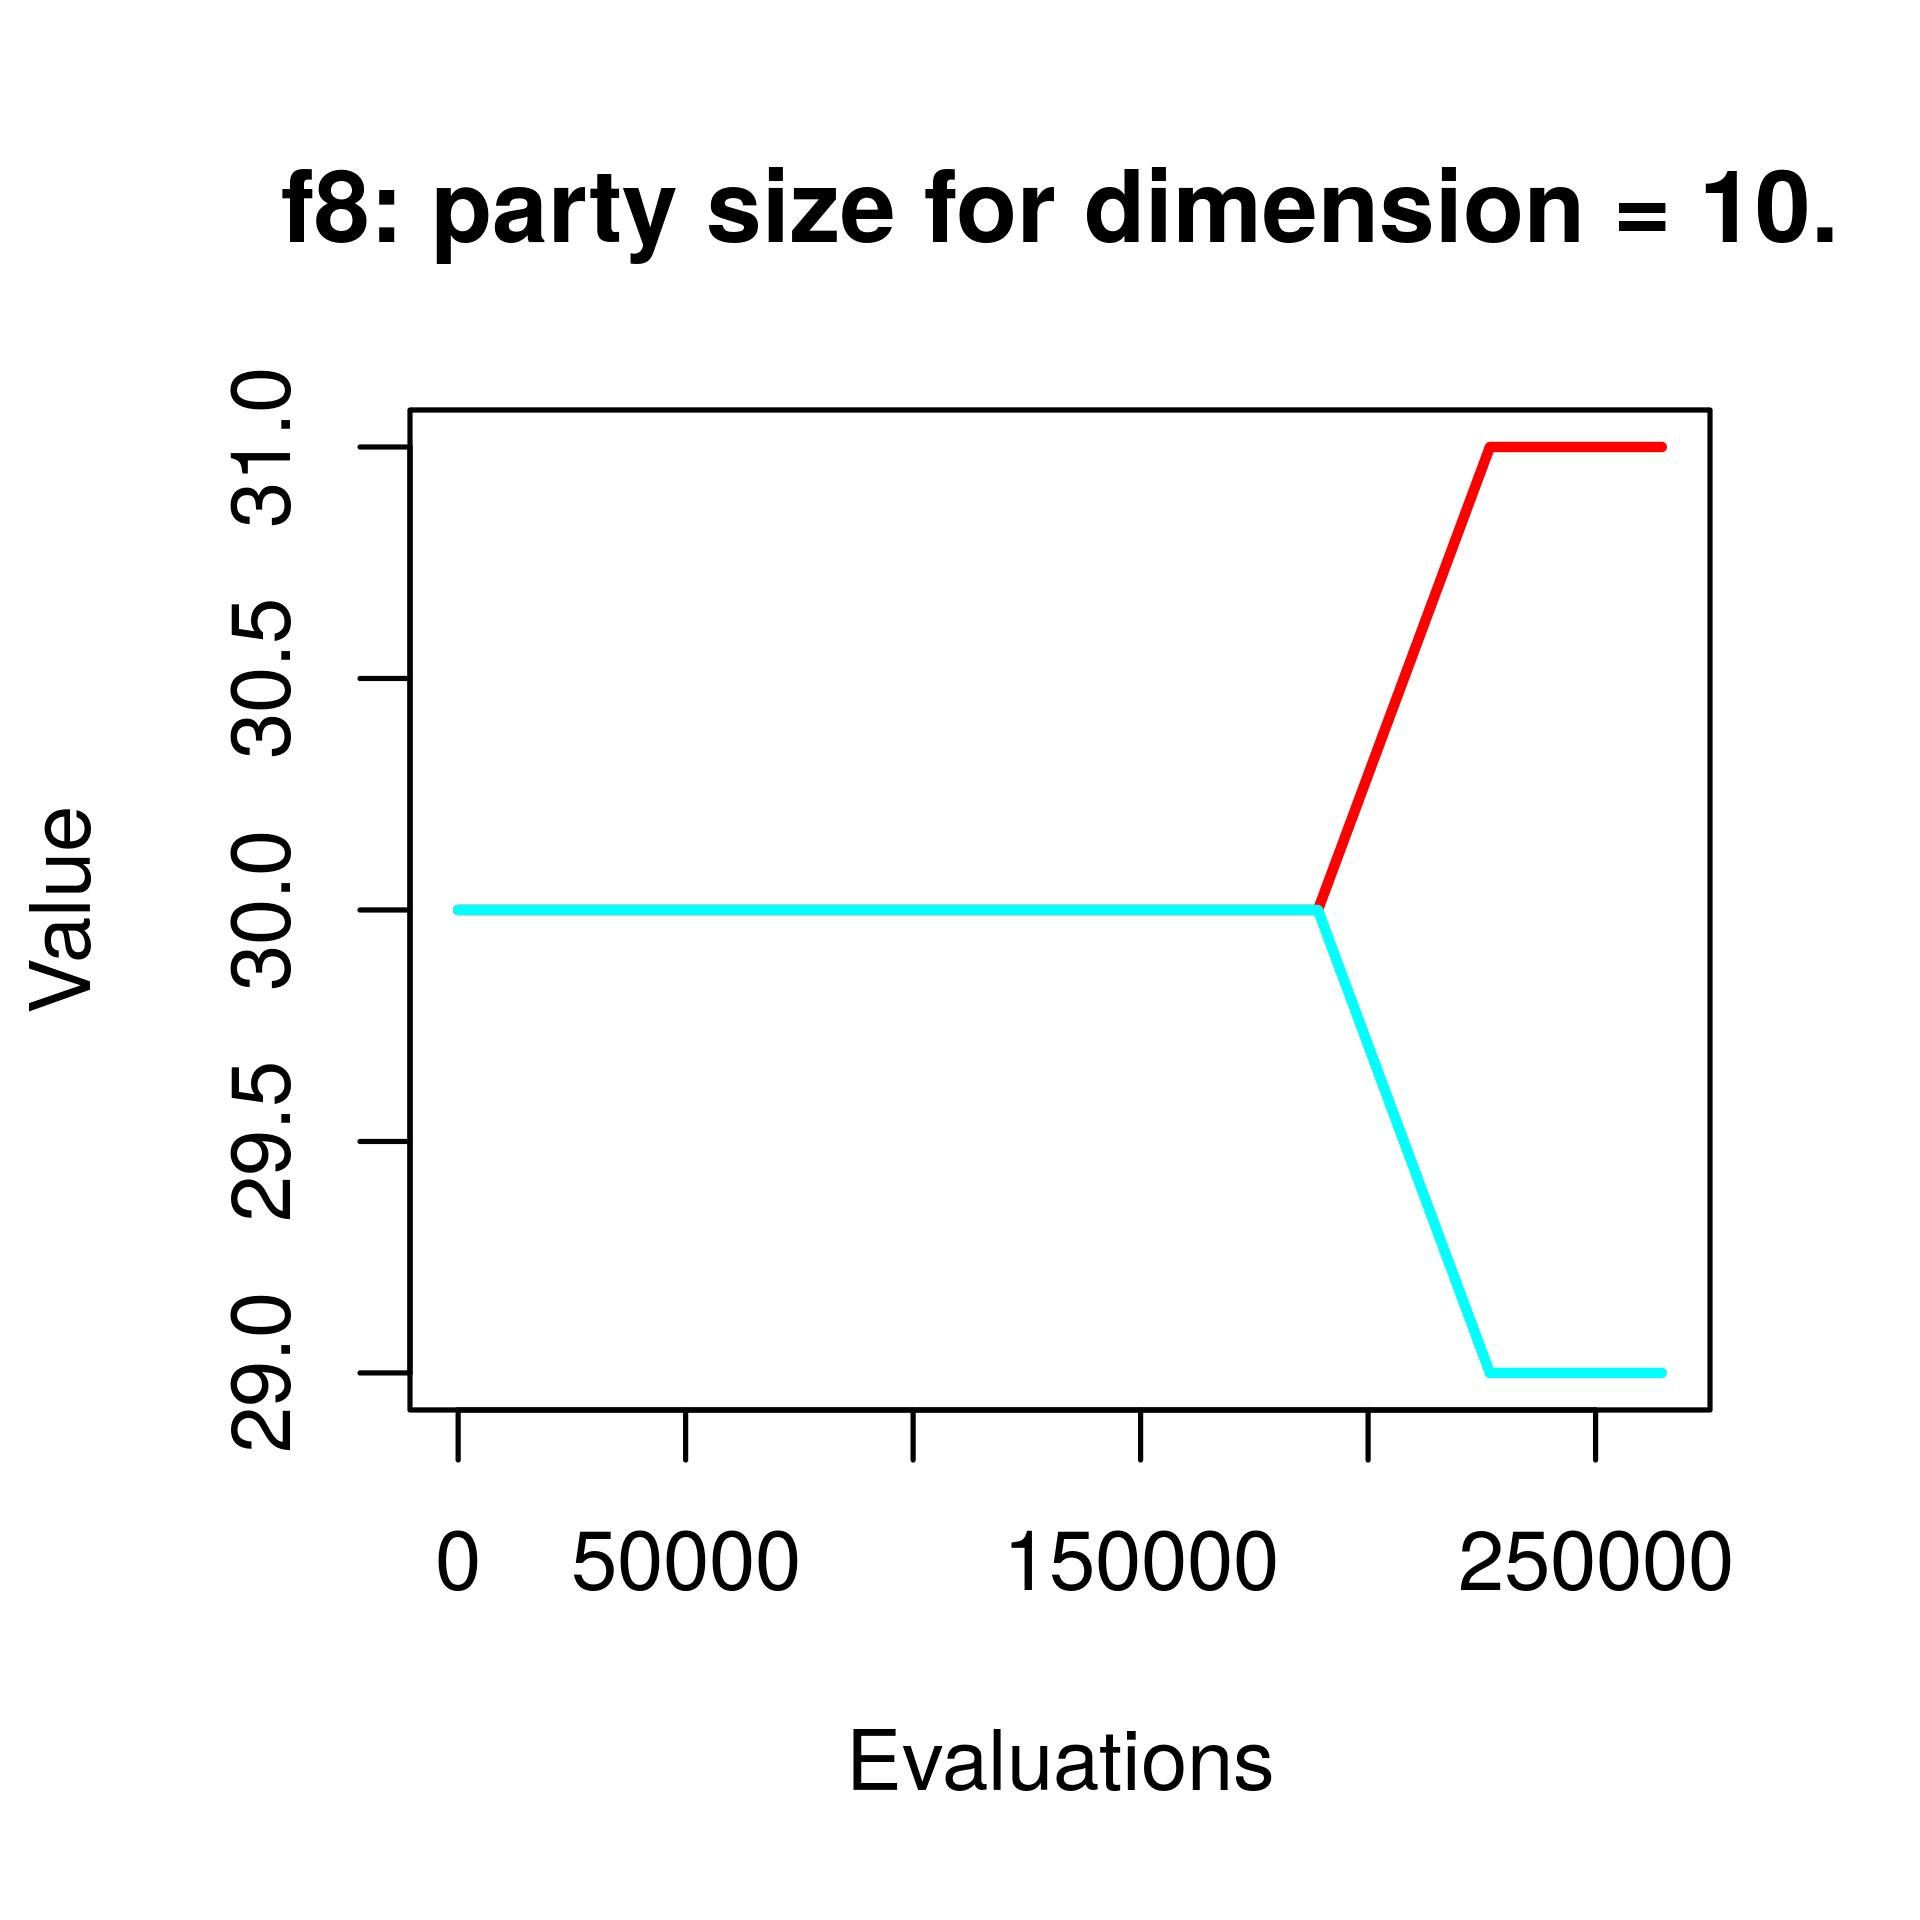
\includegraphics[width=\textwidth]{Imagenes/f8_convergence_10.jpg}
				\caption{Gráfica que representa el número de individuos del partido mayor y menor para F8.}
			\end{minipage}
		\end{figure}
		
		\noindent De nuevo, encontramos dos casos generales opuestos, con la diferencia de que, en esta ocasión, el caso en el que la población se reinicia varias veces es más acusado, puesto que, como vemos, se produce un reinicio constante en las primeras etapas del algoritmo, lo que en definitiva se traduce en buscar el mejor de entre una población de soluciones aleatorias iterativamente. Además encontramos el caso extremo opuesto, es decir, el caso en el que la población no se reinicia.
	
	\subsection{Reinicio por convergencia de la población}
	
	\noindent Esta técnica consiste en reiniciar la población cuando se detecta que la diferencia entre el mejor individuo global y el peor individuo global es menor que un umbral, lo que se traduce en una convergencia de la población en general, es decir, consideramos la población como un único conjunto que nos proporciona los marcadores de reinicio, al contrario de los criterios empleados en las técnicas anteriores, que consideraban los partidos como marcadores. Una vez más los resultados obtenidos no mejoran a los obtenidos con el algoritmo memético básico, por razones semejantes a las ya comentadas.
	
	
	\subsection{Conclusión}
		
		\noindent  A la vista de los resultados podemos concluir que, como era de esperar, la elección del umbral que supone la reinicialización de la población es determinante para el comportamiento del algoritmo, de esta forma, establecer un umbral demasiado bajo supone que la población no se reinicie y por tanto obtengamos los mismos resultados que con el algoritmo memético básico; por otra parte, establecer un umbral demasiado alto supondría, en el peor de los casos, un reinicio constante de la población, lo que, además de un sobrecoste computacional, supone cambiar radicalmente el comportamiento del algoritmo de forma que este no es capaz de explorar apropiadamente un espacio de soluciones en el que encontrar la mejor.
		

\section{Anexo 1: Funciones empleadas}

	\begin{itemize}
		
		\item Función 1 (F1): Shifted sphere
		
		\item Función 2 (F2): Shifted double-sum
		
		\item Función 5 (F5): Schewfel's Problem with Global Optimum on Bounds
		
		\item Función 6 (F6): Shifted Rosenbrock's function
		
		\item Función 8 (F8): Shifted rotated Ackley's function with global optimum on bounds
		
		\item Función 9 (F9): Shifted Rastrigins function
		
		\item Función 10 (F10): Shifted rotated Rastrigins function
		
		\item Función 11 (F11): Shifted rotated Weierstras's function
		
		\item Función 13 (F13): Rosenbrocks function
		
		\item Función 14 (F14): Shifted rotated expanded Schaffers F6
		
		\item Función 17 (F17): Rotated hybrid composition function F16 with noise
		
		\item Función 24 (F24): Rotated hybrid composition function
		
	\end{itemize}
	
	
	
	

\end{document}

\grid

		\begin{table}[h]
			\centering
			\setlength{\arrayrulewidth}{1mm}
			\setlength{\tabcolsep}{10pt}
			\renewcommand{\arraystretch}{1.5}
			
			\rowcolors{2}{gray!25}{white}
			\begin{tabular}{ >{\centering\arraybackslash}m{1.3cm}  >{\centering\arraybackslash}m{1.3cm}  >{\centering\arraybackslash}m{2cm}   >{\centering\arraybackslash}m{1.3cm}  >{\centering\arraybackslash}m{1.6cm}  >{\centering\arraybackslash}m{2cm}  }
				\hline
				\rowcolor{black}
				\multicolumn{6}{c}{\bf \color{white}{Algoritmo Greedy}}\\
				\hline
				\rowcolor{gray!50}
				\textbf{Caso} & \textbf{Desv} & \textbf{Tiempo} & \textbf{Caso} & \textbf{Desv} & \textbf{Tiempo} \\
				chr20b &   &   & sko100a  &   &   \\
				chr22a &   &   & sko100b  &   &   \\
				els19 &   &   & sko100c  &   &   \\
				esc32b &   &   & sko100d  &   &   \\
				kra30b &   &   & sko100e  &   &   \\
				lipa90b &   &   & tai30  &   &   \\
				nug25 &   &   & tai50  &   &   \\
				sko56 &   &   & tai60  &   &   \\
				sko64 &   &   & tai256  &   &   \\
				sko72 &   &   & tho150  &   &   \\
				\hline
				
			\end{tabular}
			
		\end{table}